% ****** Start of file apssamp.tex ******
%DIF LATEXDIFF DIFFERENCE FILE
%DIF DEL main.tex      Wed Jul 22 18:35:36 2026
%DIF ADD main_TN.tex   Thu Jul 23 15:49:43 2026
%
%   This file is part of the APS files in the REVTeX 4.2 distribution.
%   Version 4.2a of REVTeX, December 2014
%
%   Copyright (c) 2014 The American Physical Society.
%
%   See the REVTeX 4 README file for restrictions and more information.
%
% TeX'ing this file requires that you have AMS-LaTeX 2.0 installed
% as well as the rest of the prerequisites for REVTeX 4.2
%
% See the REVTeX 4 README file
% It also requires running BibTeX. The commands are as follows:
%
%  1)  latex apssamp.tex
%  2)  bibtex apssamp
%  3)  latex apssamp.tex
%  4)  latex apssamp.tex
%
\documentclass[%
 reprint,
superscriptaddress,
%groupedaddress,
%unsortedaddress,
%runinaddress,
%frontmatterverbose,
%preprint,
%preprintnumbers,
%nofootinbib,
%nobibnotes,
%bibnotes,
 amsmath,amssymb,
 aps,
%pra,
%prb,
%rmp,
%prstab,
%prstper,
floatfix,
]{revtex4-2}

\usepackage{graphicx}% Include figure files
\usepackage{dcolumn}% Align table columns on decimal point
\usepackage{bm}% bold math
\usepackage{comment}
% \usepackage{luatexja}
\usepackage{enumitem}
\usepackage[version=4]{mhchem}
\usepackage[hidelinks]{hyperref}% add hypertext capabilities
%\usepackage[mathlines]{lineno}% Enable numbering of text and display math
%\linenumbers\relax % Commence numbering lines

%\usepackage[showframe,%Uncomment any one of the following lines to test
%%scale=0.7, marginratio={1:1, 2:3}, ignoreall,% default settings
%%text={7in,10in},centering,
%%margin=1.5in,
%%total={6.5in,8.75in}, top=1.2in, left=0.9in, includefoot,
%%height=10in,a5paper,hmargin={3cm,0.8in},
%]{geometry}
\newcommand{\He}{$^3$He }
\newcommand{\Hensf}{$^3$He-NSF}
%DIF PREAMBLE EXTENSION ADDED BY LATEXDIFF
%DIF UNDERLINE PREAMBLE %DIF PREAMBLE
\RequirePackage[normalem]{ulem} %DIF PREAMBLE
\RequirePackage{color}\definecolor{RED}{rgb}{1,0,0}\definecolor{BLUE}{rgb}{0,0,1} %DIF PREAMBLE
\providecommand{\DIFaddtex}[1]{{\protect\color{blue}\uwave{#1}}} %DIF PREAMBLE
\providecommand{\DIFdeltex}[1]{{\protect\color{red}\sout{#1}}}                      %DIF PREAMBLE
%DIF SAFE PREAMBLE %DIF PREAMBLE
\providecommand{\DIFaddbegin}{} %DIF PREAMBLE
\providecommand{\DIFaddend}{} %DIF PREAMBLE
\providecommand{\DIFdelbegin}{} %DIF PREAMBLE
\providecommand{\DIFdelend}{} %DIF PREAMBLE
\providecommand{\DIFmodbegin}{} %DIF PREAMBLE
\providecommand{\DIFmodend}{} %DIF PREAMBLE
%DIF FLOATSAFE PREAMBLE %DIF PREAMBLE
\providecommand{\DIFaddFL}[1]{\DIFadd{#1}} %DIF PREAMBLE
\providecommand{\DIFdelFL}[1]{\DIFdel{#1}} %DIF PREAMBLE
\providecommand{\DIFaddbeginFL}{} %DIF PREAMBLE
\providecommand{\DIFaddendFL}{} %DIF PREAMBLE
\providecommand{\DIFdelbeginFL}{} %DIF PREAMBLE
\providecommand{\DIFdelendFL}{} %DIF PREAMBLE
%DIF HYPERREF PREAMBLE %DIF PREAMBLE
\providecommand{\DIFadd}[1]{\texorpdfstring{\DIFaddtex{#1}}{#1}} %DIF PREAMBLE
\providecommand{\DIFdel}[1]{\texorpdfstring{\DIFdeltex{#1}}{}} %DIF PREAMBLE
\newcommand{\DIFscaledelfig}{0.5}
%DIF HIGHLIGHTGRAPHICS PREAMBLE %DIF PREAMBLE
\RequirePackage{settobox} %DIF PREAMBLE
\RequirePackage{letltxmacro} %DIF PREAMBLE
\newsavebox{\DIFdelgraphicsbox} %DIF PREAMBLE
\newlength{\DIFdelgraphicswidth} %DIF PREAMBLE
\newlength{\DIFdelgraphicsheight} %DIF PREAMBLE
% store original definition of \includegraphics %DIF PREAMBLE
\LetLtxMacro{\DIFOincludegraphics}{\includegraphics} %DIF PREAMBLE
\newcommand{\DIFaddincludegraphics}[2][]{{\color{blue}\fbox{\DIFOincludegraphics[#1]{#2}}}} %DIF PREAMBLE
\newcommand{\DIFdelincludegraphics}[2][]{% %DIF PREAMBLE
\sbox{\DIFdelgraphicsbox}{\DIFOincludegraphics[#1]{#2}}% %DIF PREAMBLE
\settoboxwidth{\DIFdelgraphicswidth}{\DIFdelgraphicsbox} %DIF PREAMBLE
\settoboxtotalheight{\DIFdelgraphicsheight}{\DIFdelgraphicsbox} %DIF PREAMBLE
\scalebox{\DIFscaledelfig}{% %DIF PREAMBLE
\parbox[b]{\DIFdelgraphicswidth}{\usebox{\DIFdelgraphicsbox}\\[-\baselineskip] \rule{\DIFdelgraphicswidth}{0em}}\llap{\resizebox{\DIFdelgraphicswidth}{\DIFdelgraphicsheight}{% %DIF PREAMBLE
\setlength{\unitlength}{\DIFdelgraphicswidth}% %DIF PREAMBLE
\begin{picture}(1,1)% %DIF PREAMBLE
\thicklines\linethickness{2pt} %DIF PREAMBLE
{\color[rgb]{1,0,0}\put(0,0){\framebox(1,1){}}}% %DIF PREAMBLE
{\color[rgb]{1,0,0}\put(0,0){\line( 1,1){1}}}% %DIF PREAMBLE
{\color[rgb]{1,0,0}\put(0,1){\line(1,-1){1}}}% %DIF PREAMBLE
\end{picture}% %DIF PREAMBLE
}\hspace*{3pt}}} %DIF PREAMBLE
} %DIF PREAMBLE
\LetLtxMacro{\DIFOaddbegin}{\DIFaddbegin} %DIF PREAMBLE
\LetLtxMacro{\DIFOaddend}{\DIFaddend} %DIF PREAMBLE
\LetLtxMacro{\DIFOdelbegin}{\DIFdelbegin} %DIF PREAMBLE
\LetLtxMacro{\DIFOdelend}{\DIFdelend} %DIF PREAMBLE
\DeclareRobustCommand{\DIFaddbegin}{\DIFOaddbegin \let\includegraphics\DIFaddincludegraphics} %DIF PREAMBLE
\DeclareRobustCommand{\DIFaddend}{\DIFOaddend \let\includegraphics\DIFOincludegraphics} %DIF PREAMBLE
\DeclareRobustCommand{\DIFdelbegin}{\DIFOdelbegin \let\includegraphics\DIFdelincludegraphics} %DIF PREAMBLE
\DeclareRobustCommand{\DIFdelend}{\DIFOaddend \let\includegraphics\DIFOincludegraphics} %DIF PREAMBLE
\LetLtxMacro{\DIFOaddbeginFL}{\DIFaddbeginFL} %DIF PREAMBLE
\LetLtxMacro{\DIFOaddendFL}{\DIFaddendFL} %DIF PREAMBLE
\LetLtxMacro{\DIFOdelbeginFL}{\DIFdelbeginFL} %DIF PREAMBLE
\LetLtxMacro{\DIFOdelendFL}{\DIFdelendFL} %DIF PREAMBLE
\DeclareRobustCommand{\DIFaddbeginFL}{\DIFOaddbeginFL \let\includegraphics\DIFaddincludegraphics} %DIF PREAMBLE
\DeclareRobustCommand{\DIFaddendFL}{\DIFOaddendFL \let\includegraphics\DIFOincludegraphics} %DIF PREAMBLE
\DeclareRobustCommand{\DIFdelbeginFL}{\DIFOdelbeginFL \let\includegraphics\DIFdelincludegraphics} %DIF PREAMBLE
\DeclareRobustCommand{\DIFdelendFL}{\DIFOaddendFL \let\includegraphics\DIFOincludegraphics} %DIF PREAMBLE
%DIF COLORLISTINGS PREAMBLE %DIF PREAMBLE
\RequirePackage{listings} %DIF PREAMBLE
\RequirePackage{color} %DIF PREAMBLE
\lstdefinelanguage{DIFcode}{ %DIF PREAMBLE
%DIF DIFCODE_UNDERLINE %DIF PREAMBLE
  moredelim=[il][\color{red}\sout]{\%DIF\ <\ }, %DIF PREAMBLE
  moredelim=[il][\color{blue}\uwave]{\%DIF\ >\ } %DIF PREAMBLE
} %DIF PREAMBLE
\lstdefinestyle{DIFverbatimstyle}{ %DIF PREAMBLE
	language=DIFcode, %DIF PREAMBLE
	basicstyle=\ttfamily, %DIF PREAMBLE
	columns=fullflexible, %DIF PREAMBLE
	keepspaces=true %DIF PREAMBLE
} %DIF PREAMBLE
\lstnewenvironment{DIFverbatim}{\lstset{style=DIFverbatimstyle}}{} %DIF PREAMBLE
\lstnewenvironment{DIFverbatim*}{\lstset{style=DIFverbatimstyle,showspaces=true}}{} %DIF PREAMBLE
%DIF END PREAMBLE EXTENSION ADDED BY LATEXDIFF

\begin{document}

\preprint{APS/123-QED}

% \title{Manuscript Title:\\with Forced Linebreak}% Force line breaks with \\
\title{Polarized neutron diffraction with \textit{ex-situ} $^3$He neutron spin filter and two-dimensional detector for a complex incommensurate magnetic order}% Force line breaks with \\


\author{S.~Takahashi}
\affiliation{Institute for Solid State Physics, The University of Tokyo, Kashiwa, Chiba 277-8581, Japan}
\affiliation{J-PARC Center, Japan Atomic Energy Agency, 2-4 Shirakata, Tokai, Ibaraki 319-1195, Japan}

\author{Y.~Osawa}
\affiliation{Institute for Solid State Physics, The University of Tokyo, Kashiwa, Chiba 277-8581, Japan}

\author{R.~Kobayashi}
\affiliation{J-PARC Center, Japan Atomic Energy Agency, 2-4 Shirakata, Tokai, Ibaraki 319-1195, Japan}

\author{T.~Ino}
\affiliation{Institute of Materials Structure Science, High Energy Accelerator Research Organization, 1-1 Oho, Tsukuba, Ibaraki 305-0801, Japan}

\author{H.~Saito}
\affiliation{Institute for Solid State Physics, The University of Tokyo, Kashiwa, Chiba 277-8581, Japan}

\author{T.~Kawasaki}
\affiliation{J-PARC Center, Japan Atomic Energy Agency, 2-4 Shirakata, Tokai, Ibaraki 319-1195, Japan}

\author{T.~Oku}
\affiliation{J-PARC Center, Japan Atomic Energy Agency, 2-4 Shirakata, Tokai, Ibaraki 319-1195, Japan}
\affiliation{Ibaraki University, 2-1-1 Bunkyo, mito, Ibaraki 310-8512, Japan}

\author{T.~Nakamura}
\affiliation{J-PARC Center, Japan Atomic Energy Agency, 2-4 Shirakata, Tokai, Ibaraki 319-1195, Japan}

\author{Y.~Ikeda}
\affiliation{Institute for Materials Research, Tohoku University, 2-1-1 Katahira, Sendai 980-8577, Japan}

\author{M.~Fujita}
\affiliation{Institute for Materials Research, Tohoku University, 2-1-1 Katahira, Sendai 980-8577, Japan}

\author{Y.~Tokunaga}
\affiliation{Department of Advanced Materials Science, University of Tokyo, Kashiwa 277-8561, Japan}

\author{T.~Arima}
\affiliation{Department of Advanced Materials Science, University of Tokyo, Kashiwa 277-8561, Japan}
\affiliation{RIKEN Center for Emergent Matter Science, Wako, Saitama 351-0198, Japan}

\author{T.~Nakajima}
\affiliation{Institute for Solid State Physics, The University of Tokyo, Kashiwa, Chiba 277-8581, Japan}
\affiliation{Institute of Materials Structure Science, High Energy Accelerator Research Organization, 1-1 Oho, Tsukuba, Ibaraki 305-0801, Japan}
\affiliation{RIKEN Center for Emergent Matter Science, Wako, Saitama 351-0198, Japan}

\begin{center}
    last updated : \today
\end{center}

\begin{abstract}
Polarized neutron scattering has been widely used for studying magnetic orders in condensed matter.
One of the typical setups for this technique is a triple-axis spectrometer with a ferromagnetic single-crystal monochromator and analyzer, which is suited for point-by-point measurements on a horizontal scattering plane.
However, this setup cannot fully meet the demands of recent studies on complex magnetic orders with emergent cross-correlated phenomena.
For instance, multiferroics, magnetic skyrmions, and other topologically-nontrivial magnetic orders tend to have incommensurate magnetic modulation vectors running along various directions in reciprocal space, which cannot be captured by measurements restricted to the horizontal scattering plane.
To overcome these limitations, we developed an experimental setup combining a \He neutron spin filter (\Hensf) and a two-dimensional (2D) detector, which enables us to analyze polarization of neutron scattered in out-of-plane direction.
We also established a data reduction procedure to convert the 2D intensity maps into three-dimensional intensity distributions in the reciprocal space with corrections of the imperfection in \He polarization.
This method was applied to single-crystal diffraction measurements on the multiferroic material \ce{Mn3WO6}, which exhibits complex incommensurate magnetic orders.
We successfully observed polarization-dependent intensities of out-of-plane incommensurate magnetic reflections, demonstrating the effectiveness of the present method for analyzing complex magnetic structures.
\end{abstract}

%\keywords{Suggested keywords}%Use showkeys class option if keyword
%display desired
\maketitle
\section{Introduction}
Polarized neutron scattering is a powerful technique for investigating magnetic order and excitations in condensed matter.
This capability arises \DIFdelbegin \DIFdel{because neutrons interact directly }\DIFdelend \DIFaddbegin \DIFadd{from the magnetic moment of neutron, which directly interacts }\DIFaddend with magnetic moments in the material through the magnetic \DIFdelbegin \DIFdel{dipole }\DIFdelend \DIFaddbegin \DIFadd{dipole-dipole }\DIFaddend interaction.
By analyzing the spin states of neutrons before and after scattering, \DIFdelbegin \DIFdel{magnetic scattering can be separated }\DIFdelend \DIFaddbegin \DIFadd{one can separate magnetic scattering }\DIFaddend from nuclear scattering\DIFdelbegin \DIFdel{.
The }\DIFdelend \DIFaddbegin \DIFadd{, and determine the }\DIFaddend directions of magnetic moments \DIFdelbegin \DIFdel{can also be determined}\DIFdelend \DIFaddbegin \DIFadd{in the sample}\DIFaddend .
To perform \DIFdelbegin \DIFdel{such polarization analysis, a neutron polarization device is required.
Three techniques are }\DIFdelend \DIFaddbegin \DIFadd{these meaurements, devices for controlling and probing the neutron polarization are required.
To this date, there are mainly three techniques }\DIFaddend commonly used for \DIFdelbegin \DIFdel{neutron polarization}\DIFdelend \DIFaddbegin \DIFadd{polarized neutron scattering}\DIFaddend .
The first \DIFdelbegin \DIFdel{employs Bragg reflection from a ferromagnetic single crystal }\DIFdelend \DIFaddbegin \DIFadd{one is a single crystal of ferromagnetic material}\DIFaddend , such as \DIFdelbegin \DIFdel{a Heusler crystal of \ce{Cu2MnAl}}\DIFdelend \DIFaddbegin \DIFadd{\ce{Cu2MnAl} Heusler compound.
By exploiting the nuclear-magnetic interference effect}[]\DIFadd{, a polarized monochromatic neutron beam can be obtained by a Bragg reflection of the ferromagnetic single crystal}\DIFaddend .
The second \DIFdelbegin \DIFdel{uses reflection from }\DIFdelend \DIFaddbegin \DIFadd{is }\DIFaddend a polarizing supermirror\DIFaddbegin \DIFadd{, which utilizes the difference in critical angle between the neutrons with different spin states}\DIFaddend .
The third is filtering of neutron spin state using polarized \He nuclei (\He neutron spin filter, \Hensf).
Among these techniques, \DIFdelbegin \DIFdel{polarization analysis at }\DIFdelend \DIFaddbegin \DIFadd{the ferromagnetic single-crystal monochromators and analyzers are often used in }\DIFaddend triple-axis \DIFdelbegin \DIFdel{spectrometers is often performed using Heusler crystals as the neutron polarizer and analyzer }\DIFdelend \DIFaddbegin \DIFadd{spectrometers}\DIFaddend \cite{kulda_in20_2002,faulhaber_polarized_2010,fernandez-baca_triple-axis_2008,takeda_double_2008,nakajima_polarized_2024}, as shown in Fig.~\ref{fig:introduction}(a).
%DIF >  Among these techniquesときたら、その次にはその３つのテクニックのうちどれかが文頭にこないとおかしいです。
While this type of instrument has been widely used for \DIFdelbegin \DIFdel{magnetic structure analysis, the accessible scattering vectors are for restricted to the }\DIFdelend \DIFaddbegin \DIFadd{studying the magnetic structures, accessible reflections are often restricted to a }\DIFaddend horizontal scattering plane.

In recent years, increasing attention has been paid to materials hosting complex \DIFdelbegin \DIFdel{magnetic structures.
In such materials}\DIFdelend \DIFaddbegin \DIFadd{incommensurate magnetic orders, such as spin-driven multiferroics, magnetic skyrmions and related topological magnetic orders\mbox{%DIFAUXCMD
\cite{muhlbauer_skyrmion_2009,tokura_multiferroics_2014,kanazawa_direct_2020,fujishiro_topological_2019,kurumaji_electronic_2025}}\hskip0pt%DIFAUXCMD
.
In these systems}\DIFaddend , the magnetic moments are often arranged in noncollinear or noncoplanar configurations, which can give rise to emergent cross-correlated phenomena.
\DIFdelbegin \DIFdel{Representative examples include magnetic skyrmions and spin-hedgehog lattices \mbox{%DIFAUXCMD
\cite{muhlbauer_skyrmion_2009,tokura_multiferroics_2014}}\hskip0pt%DIFAUXCMD
.
A common feature of these systemsis that their magnetic structures are often described by multiple }\DIFdelend \DIFaddbegin \DIFadd{To study these systems, it is necessary to measure magnetic satellite reflections corresponding to }\DIFaddend magnetic modulation wavevectors ($q$-vectors)\DIFaddbegin \DIFadd{, which often run along various directions in the reciprocal space}\DIFaddend .
Consequently, \DIFdelbegin \DIFdel{the associated magnetic reflections can be distributed not only within a horizontal scattering plane but throughout }\DIFdelend three-dimensional \DIFdelbegin \DIFdel{reciprocal space.
To perform polarization analysis on these reflections, a large-solid-angle polarization device }\DIFdelend \DIFaddbegin \DIFadd{explorations of the reciprocal space with two-dimensional (2D) detector is of great importance.
To realize polarization analysis in the measurements with a 2D detector, polarization devices with a large solid-angle coverage, }\DIFaddend such as \Hensf\DIFdelbegin \DIFdel{~is }\DIFdelend \DIFaddbegin \DIFadd{, are }\DIFaddend required.

\DIFdelbegin \DIFdel{As an experimental technique for elucidating such complex magnetic structures, polarized }\DIFdelend \DIFaddbegin \DIFadd{The combination of \Hensf\ and 2D detector was implemented in several }\DIFaddend small-angle neutron scattering (SANS) \DIFdelbegin \DIFdel{has been widely used \mbox{%DIFAUXCMD
\cite{muhlbauer_skyrmion_2009,kanazawa_direct_2020,fujishiro_topological_2019,kurumaji_electronic_2025}}\hskip0pt%DIFAUXCMD
.
In polarized SANS, three-dimensional polarization analysis is already realized by combining a \Hensf~and a two-dimensional (2D) detector~}\DIFdelend \DIFaddbegin \DIFadd{instruments, and was applied to the studies on complex magnetic orders}\DIFaddend \cite{singh_transition_2023,takagi_multiple-q_2018}.
In \DIFdelbegin \DIFdel{this setup}\DIFdelend \DIFaddbegin \DIFadd{SANS instruments}\DIFaddend , however, the \DIFdelbegin \DIFdel{detector and the \Hensf~are positioned directly in line with the incident beam, so the }\DIFdelend accessible region is restricted to relatively low-$Q$.
\DIFdelbegin \DIFdel{If the same }\DIFdelend \DIFaddbegin \DIFadd{To extend the accessible $Q$ range with polarization analysis to middle-$Q$ and high-$Q$ regions, a }\DIFaddend combination of \Hensf~and 2D detector \DIFaddbegin \DIFadd{placed }\DIFaddend at finite scattering angles as illustrated in Fig.~\ref{fig:introduction}(b) \DIFdelbegin \DIFdel{, polarization analysis can be extended to much higher-$Q$ regions.
This would make it possible to access a wide variety of magnetic reflections distributed throughout three-dimensional reciprocal space, including those associated with the complex magnetic structures described above.
}\DIFdelend \DIFaddbegin \DIFadd{would be necessary.
%DIF > This would make it possible to access a wide variety of magnetic reflections distributed throughout three-dimensional reciprocal space, including those associated with the complex magnetic structures described above.
}\DIFaddend Related instrumental concepts have already been reported at several neutron facilities, including POLI at MLZ~\cite{thoma_polarized_2018} and WOMBAT at ANSTO~\cite{lee_polarised_2016}.
Nevertheless, to the best of our knowledge, quantitative experimental demonstrations of polarization analysis using this type of setup remain limited.


In \DIFdelbegin \DIFdel{this work}\DIFdelend \DIFaddbegin \DIFadd{the present study}\DIFaddend , we performed \DIFdelbegin \DIFdel{polarization analysis }\DIFdelend \DIFaddbegin \DIFadd{polarized neutron diffraction measurements }\DIFaddend combining a \Hensf~and a 2D detector \DIFdelbegin \DIFdel{on the polarized neutron triple-axis spectrometer PONTA at }\DIFdelend \DIFaddbegin \DIFadd{at the 5G beamport in }\DIFaddend JRR-3.
\DIFdelbegin \DIFdel{Polarized neutron diffraction experiments on \ce{Mn3WO6} were performed using this setup.
\ce{Mn3WO6} is a multiferroic material with a ferroaxial crystal structure belonging to the R$\bar{3}$ space group \mbox{%DIFAUXCMD
\cite{maignan_spin-induced_2020}}\hskip0pt%DIFAUXCMD
.
This system undergoes an antiferromagnetic phase transition at 24.5 K and exhibits spontaneous electric polarization below 22 K.
In this study, polarization analysis was performed }\DIFdelend \DIFaddbegin \DIFadd{This paper mainly describes the experimental setups and procedures of corrections for the effect of imperfect neutron polarization.
We also performed polarized neutron diffraction on a single crystal of \ce{Mn3WO6}, which exhibits incommensurate magnetic orders.
The crystal structure of this compound belongs to the space group of $R\bar{3}$, and displays two magnetically ordered phases at low temperatures\mbox{%DIFAUXCMD
\cite{maignan_spin-induced_2020}}\hskip0pt%DIFAUXCMD
.
As we describe in the following sections, we focus on the data measured }\DIFaddend at 23 K, \DIFdelbegin \DIFdel{just below the antiferromagnetic transition.
This paper mainly describes the experimental method and the data-analysis procedure}\DIFdelend \DIFaddbegin \DIFadd{which is in the high temperature magnetic phase.
We performed polarization analysis for magnetic reflections which were slightly shifted from the horizontal plane}\DIFaddend .
The details of the magnetic structure will be reported in a separate paper.


\begin{figure}[h]
    \centering
    \DIFdelbeginFL %DIFDELCMD < 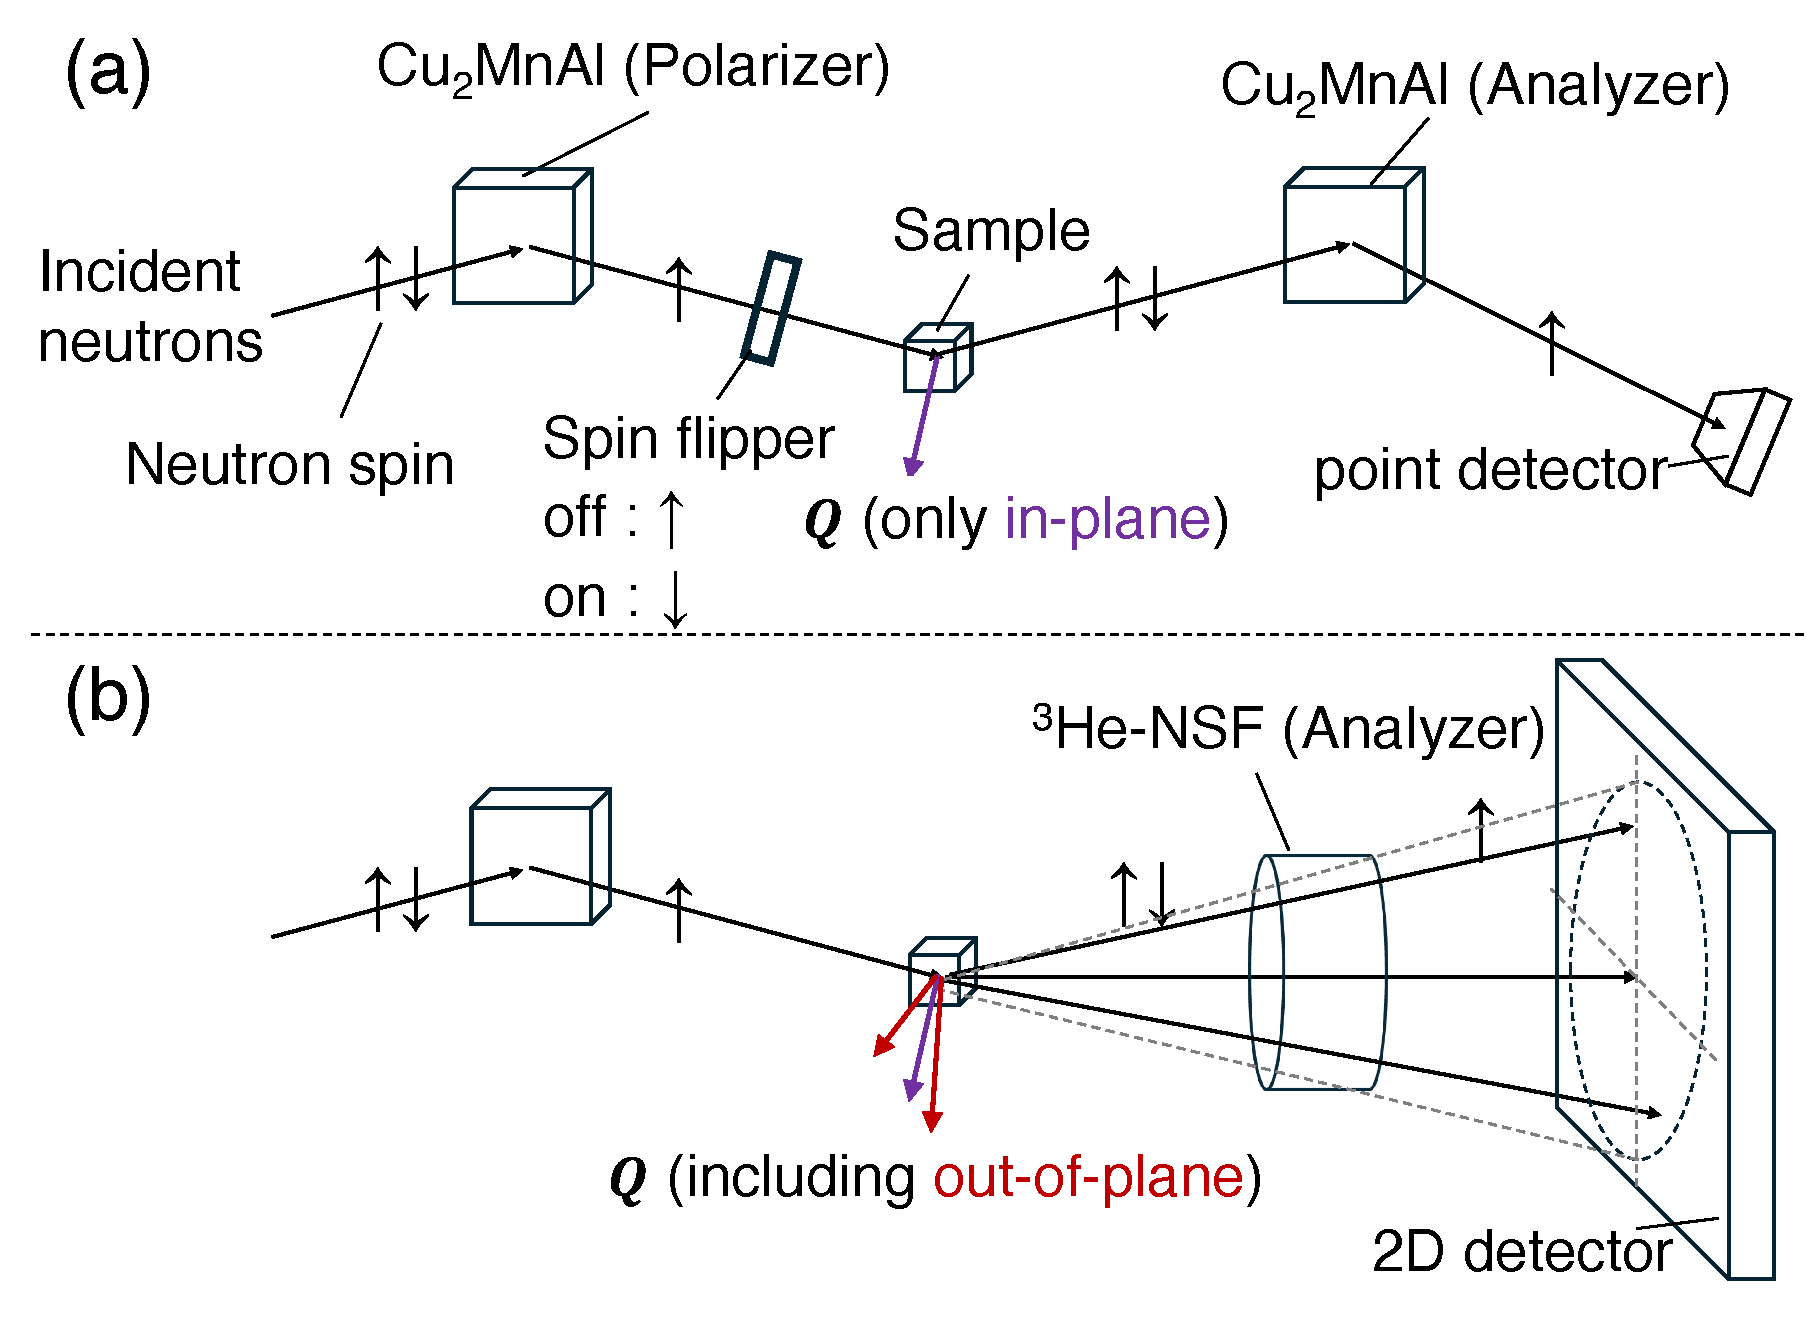
\includegraphics[width=8.5cm]{figure/Figure1_v9.pdf}
%DIFDELCMD <     %%%
\DIFdelendFL \DIFaddbeginFL 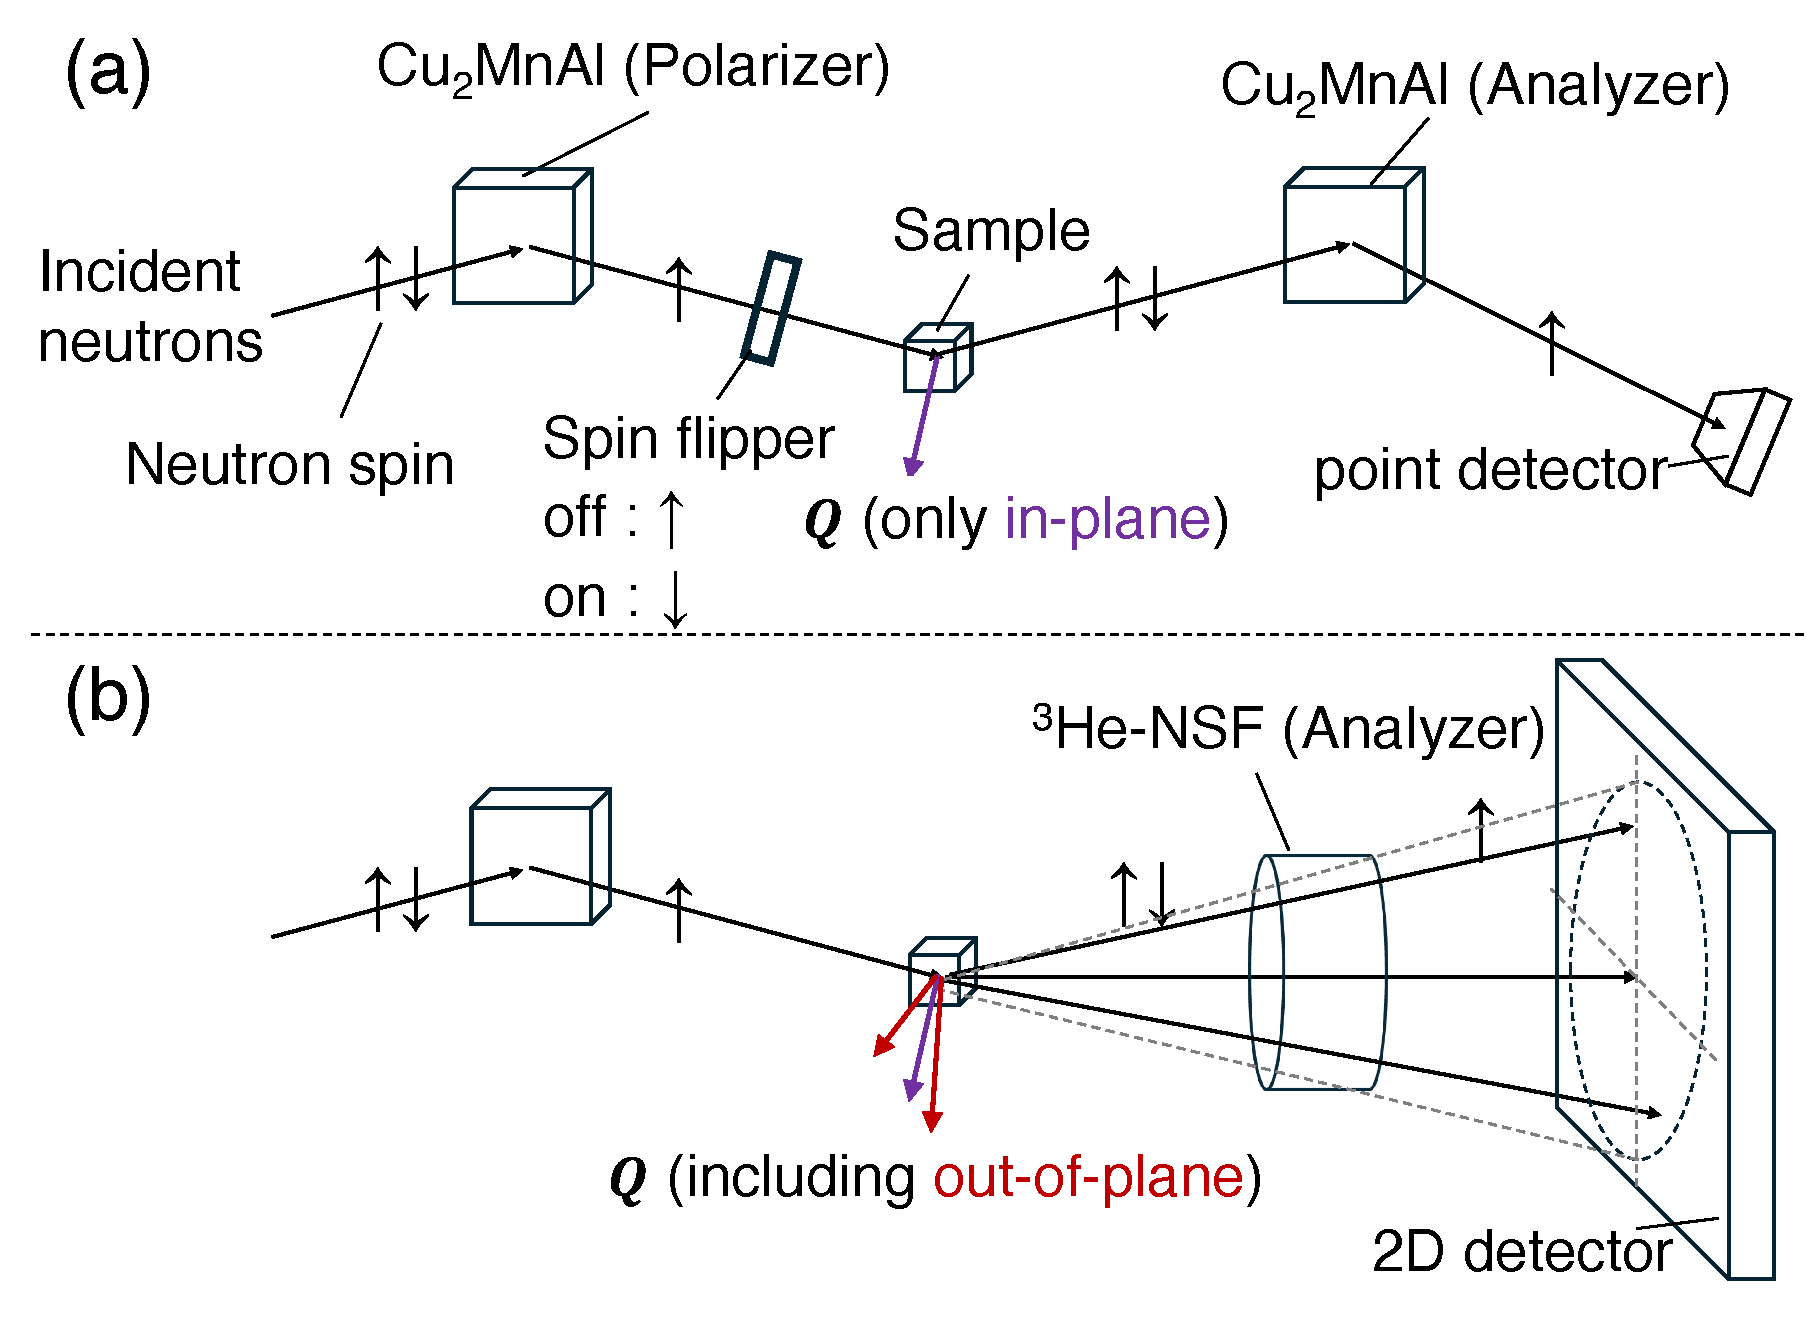
\includegraphics[width=8.5cm]{figure/Figure1_v9.pdf}
    \DIFaddendFL \caption{Schematic illustrations comparing neutron polarization analysis techniques.
(a) Conventional setup using Heusler crystals for both polarizer and analyzer, where only in-plane scattered neutrons are detected by a point detector.
(b) Polarization analysis setup combining a \Hensf~and a 2D detector, enabling detection of both in-plane and out-of-plane scattered neutrons.}
    \label{fig:introduction}
\end{figure}


\section{Experimental details}


\subsection{Setup}
% 一般論
\DIFdelbegin \DIFdel{PONTA is one of the polarized neutron triple-axis spectrometers at JRR-3.
It has }\DIFdelend \DIFaddbegin \DIFadd{The 5G beamport in JRR-3 is normally operated with the POlarized Neutron Triple-Axis spectrometer PONTA, which }\DIFaddend a longitudinal polarization analysis option \DIFdelbegin \DIFdel{~\mbox{%DIFAUXCMD
\cite{nakajima_polarized_2024}}\hskip0pt%DIFAUXCMD
.
In this option, both the incident and scattered neutrons are polarized and analyzed by a \ce{Cu2MnAl} Heusler crystal }\DIFdelend \DIFaddbegin \DIFadd{with conventional Heusler }\DIFaddend monochromator and analyzer\DIFaddbegin \DIFadd{~\mbox{%DIFAUXCMD
\cite{nakajima_polarized_2024}}\hskip0pt%DIFAUXCMD
}\DIFaddend .
In the present experiment, the Heusler analyzer and the point detector were replaced with a \Hensf\DIFaddbegin \DIFadd{\ }\DIFaddend and a 2D detector.
\DIFaddbegin \DIFadd{The polarized incident neutron beam with the energy of 14.7 meV was obtained by the Heusler monochromator.
The higher-order reflections from the monochromator were suppressed by the pyrolytic graphite filter placed between the monochromator and the sample.
}\DIFaddend Fig.~\ref{fig:Setup} shows an overview of the experimental setup from the sample to the detector.
Scattered neutrons were detected using a scintillation-type 2D detector employing wavelength-shifting-fiber readout~\cite{nakamura_large-area_2012}.
The active area is \(256 \times 256\) mm$^2$ (64 ch $\times$ 64 ch), corresponding to a channel pitch of 4 mm/ch.
The detector was positioned at an angle of \DIFdelbegin \DIFdel{approximately }\DIFdelend \(32^\circ\) with respect to the incident neutron beam and remained fixed throughout the measurement.
The sample-to-detector distance was 0.915 m.
A \Hensf~was installed 0.43 m downstream of the sample between the sample and the detector.
The cylindrical \He cell had a diameter of 72 mm \DIFaddbegin \DIFadd{and length of ** mm}\DIFaddend , providing an angular acceptance of \(\pm4.0^\circ\), which covered approximately half of the central region of the detector.
To reduce the background, a \ce{B4C}-shielded neutron guide tube was installed between the \Hensf~and the detector, and \ce{B4C} shielding was also attached around the \Hensf~coil.
As described in the following section, polarization analysis of the scattered neutrons was performed by flipping the \He polarization.
Therefore, the neutron spin flipper for the incident beam was not used.

A single-crystal sample of \ce{Mn3WO6} with a volume of 8 mm$^3$ was mounted on an aluminum holder and installed in a \DIFdelbegin \DIFdel{cryostat with the scattering plane set to the $(H0L)$ plane}\DIFdelend \DIFaddbegin \DIFadd{$^4$He closed-cycle refrigerator with the $(H,0,L)$ horizontal scattering plane}\DIFaddend .
The rotation angle $\omega$ of the sample was adjustable to align the target reflection with the detector.
The Helmholtz coil was used to maintain the neutron spin polarization along the neutron flight path by applying a vertical magnetic field.
The magnetic field in the \Hensf~was oriented parallel to the beam axis, and the spins of neutrons scattered from the sample adiabatically followed the field direction, as illustrated in Fig.~\ref{fig:Setup}.
The magnetic field strength generated by both the \Hensf~coil and the Helmholtz coil was approximately 1 mT.

\begin{figure}[t]
    \centering
    \DIFdelbeginFL %DIFDELCMD < 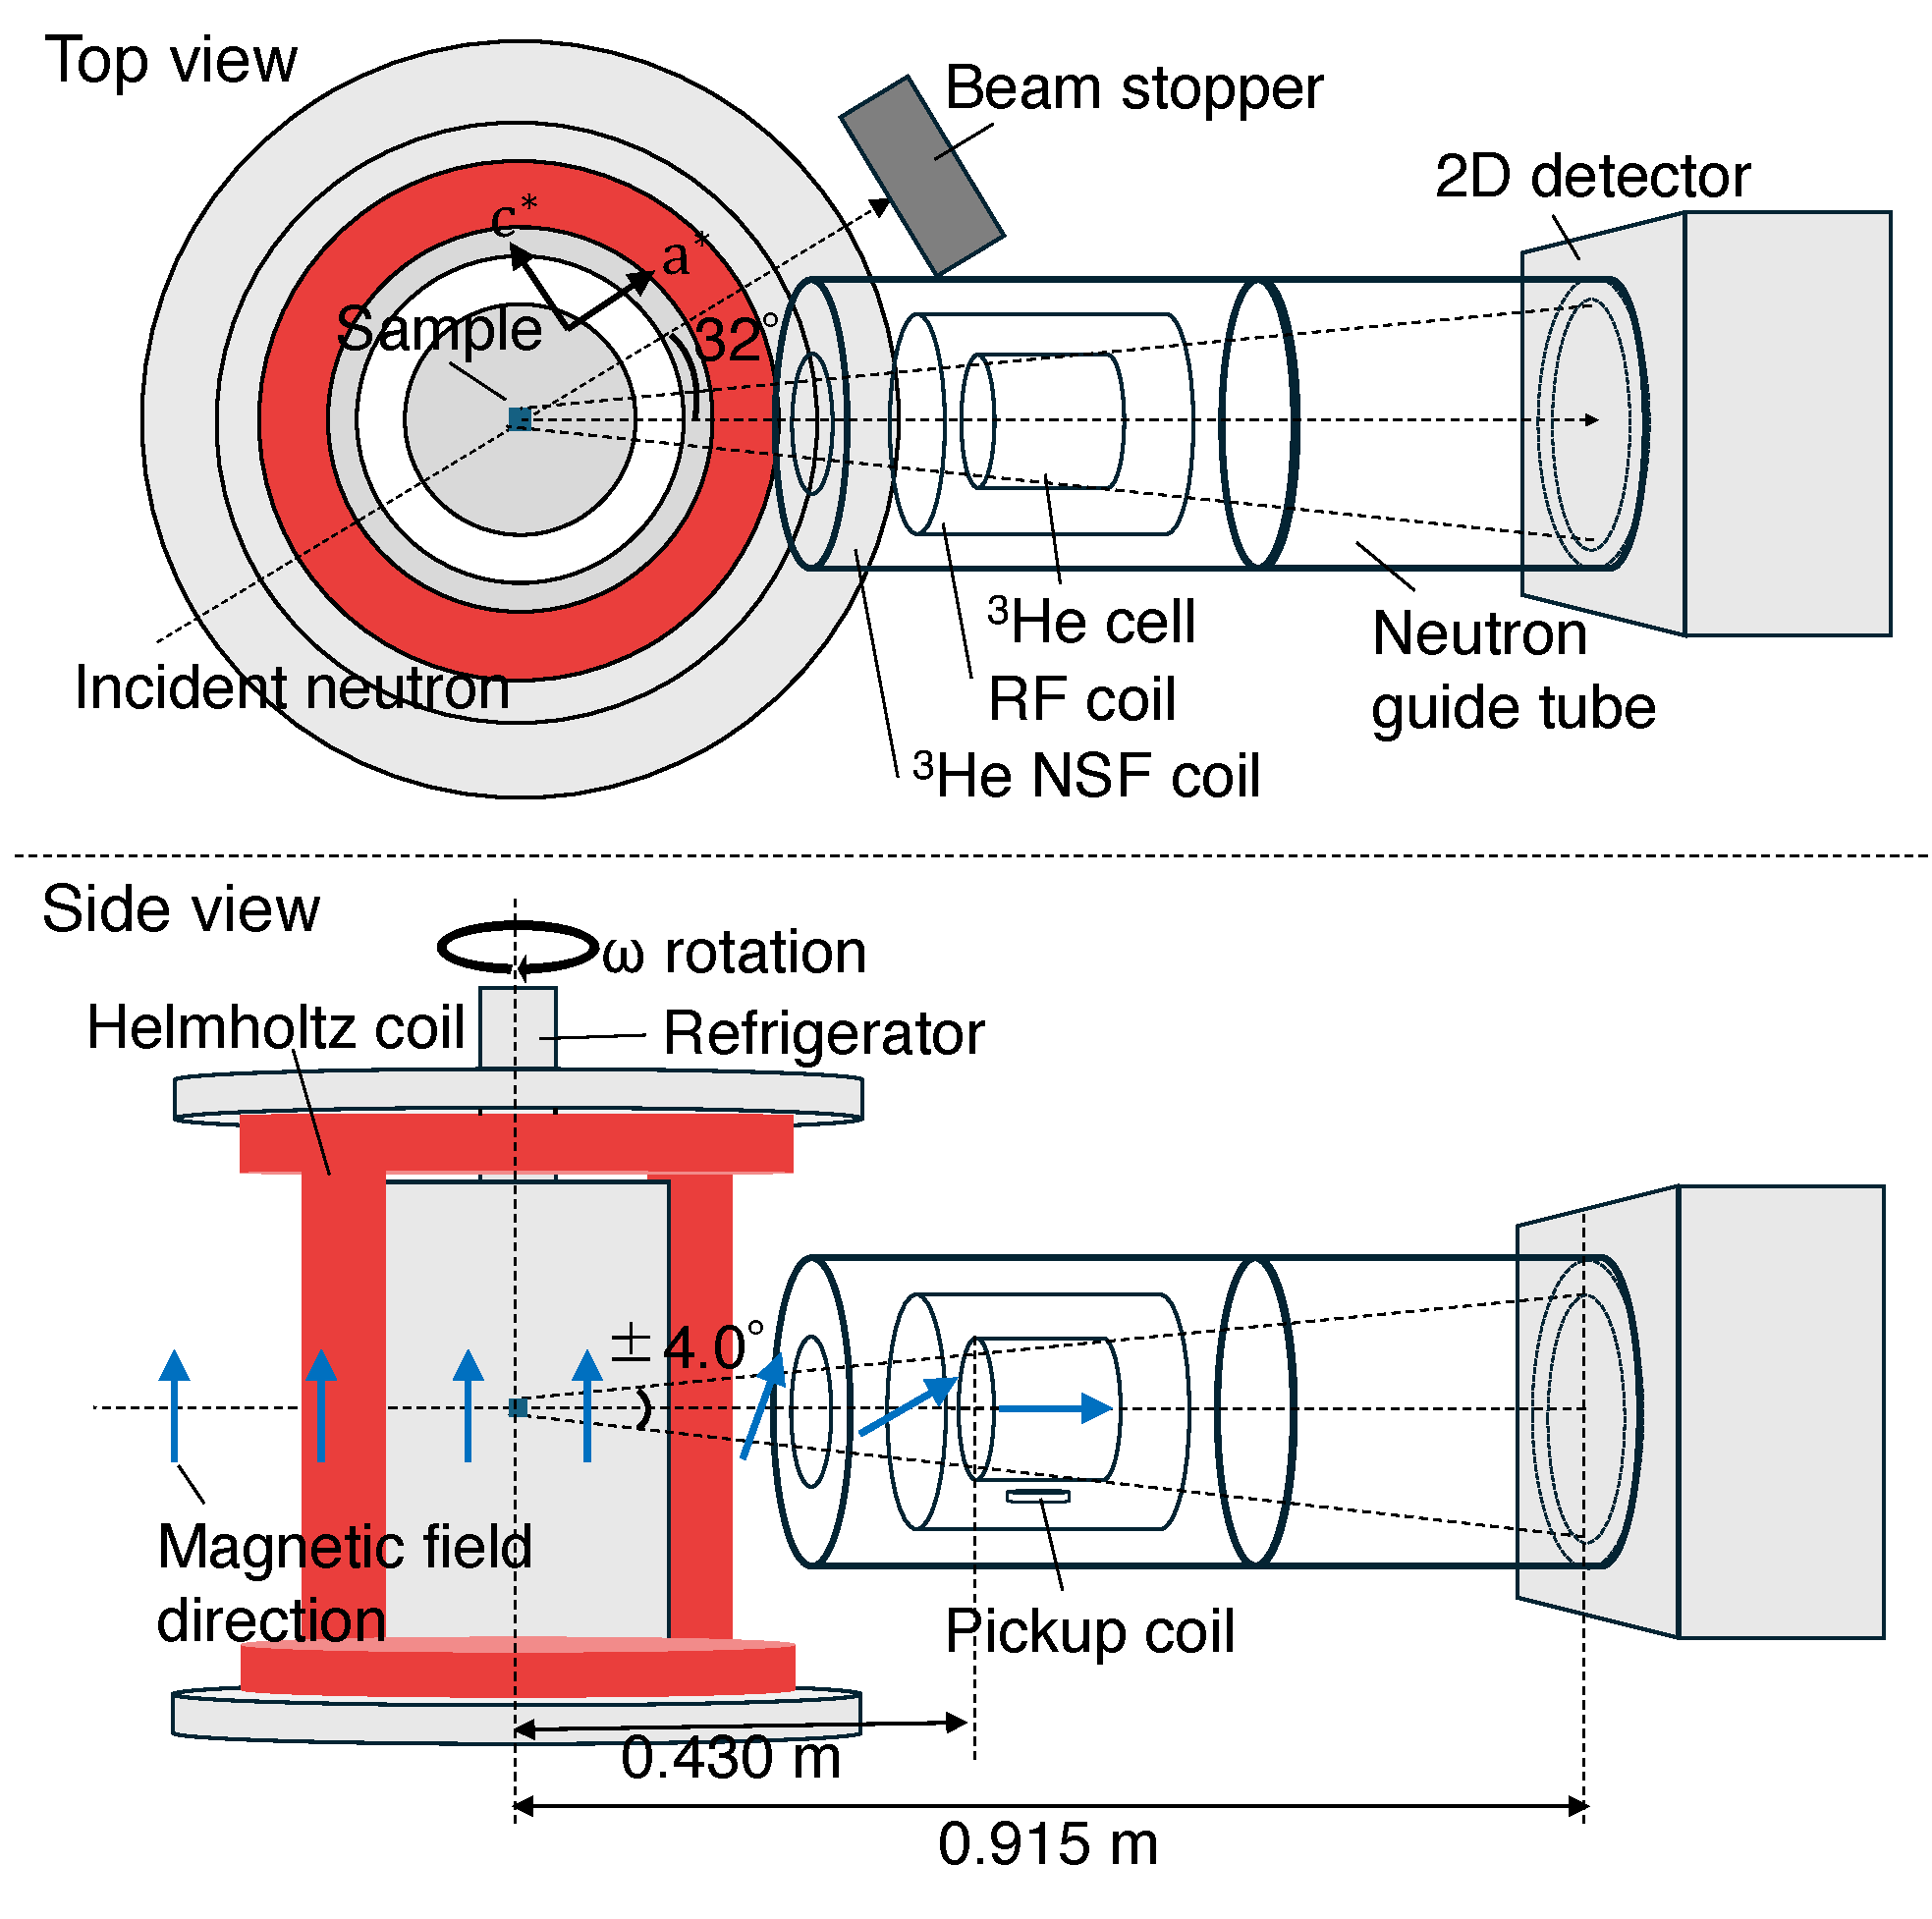
\includegraphics[width=8.5cm]{figure/Scattering_Angle_v7.pdf}
%DIFDELCMD <     %%%
\DIFdelendFL \DIFaddbeginFL 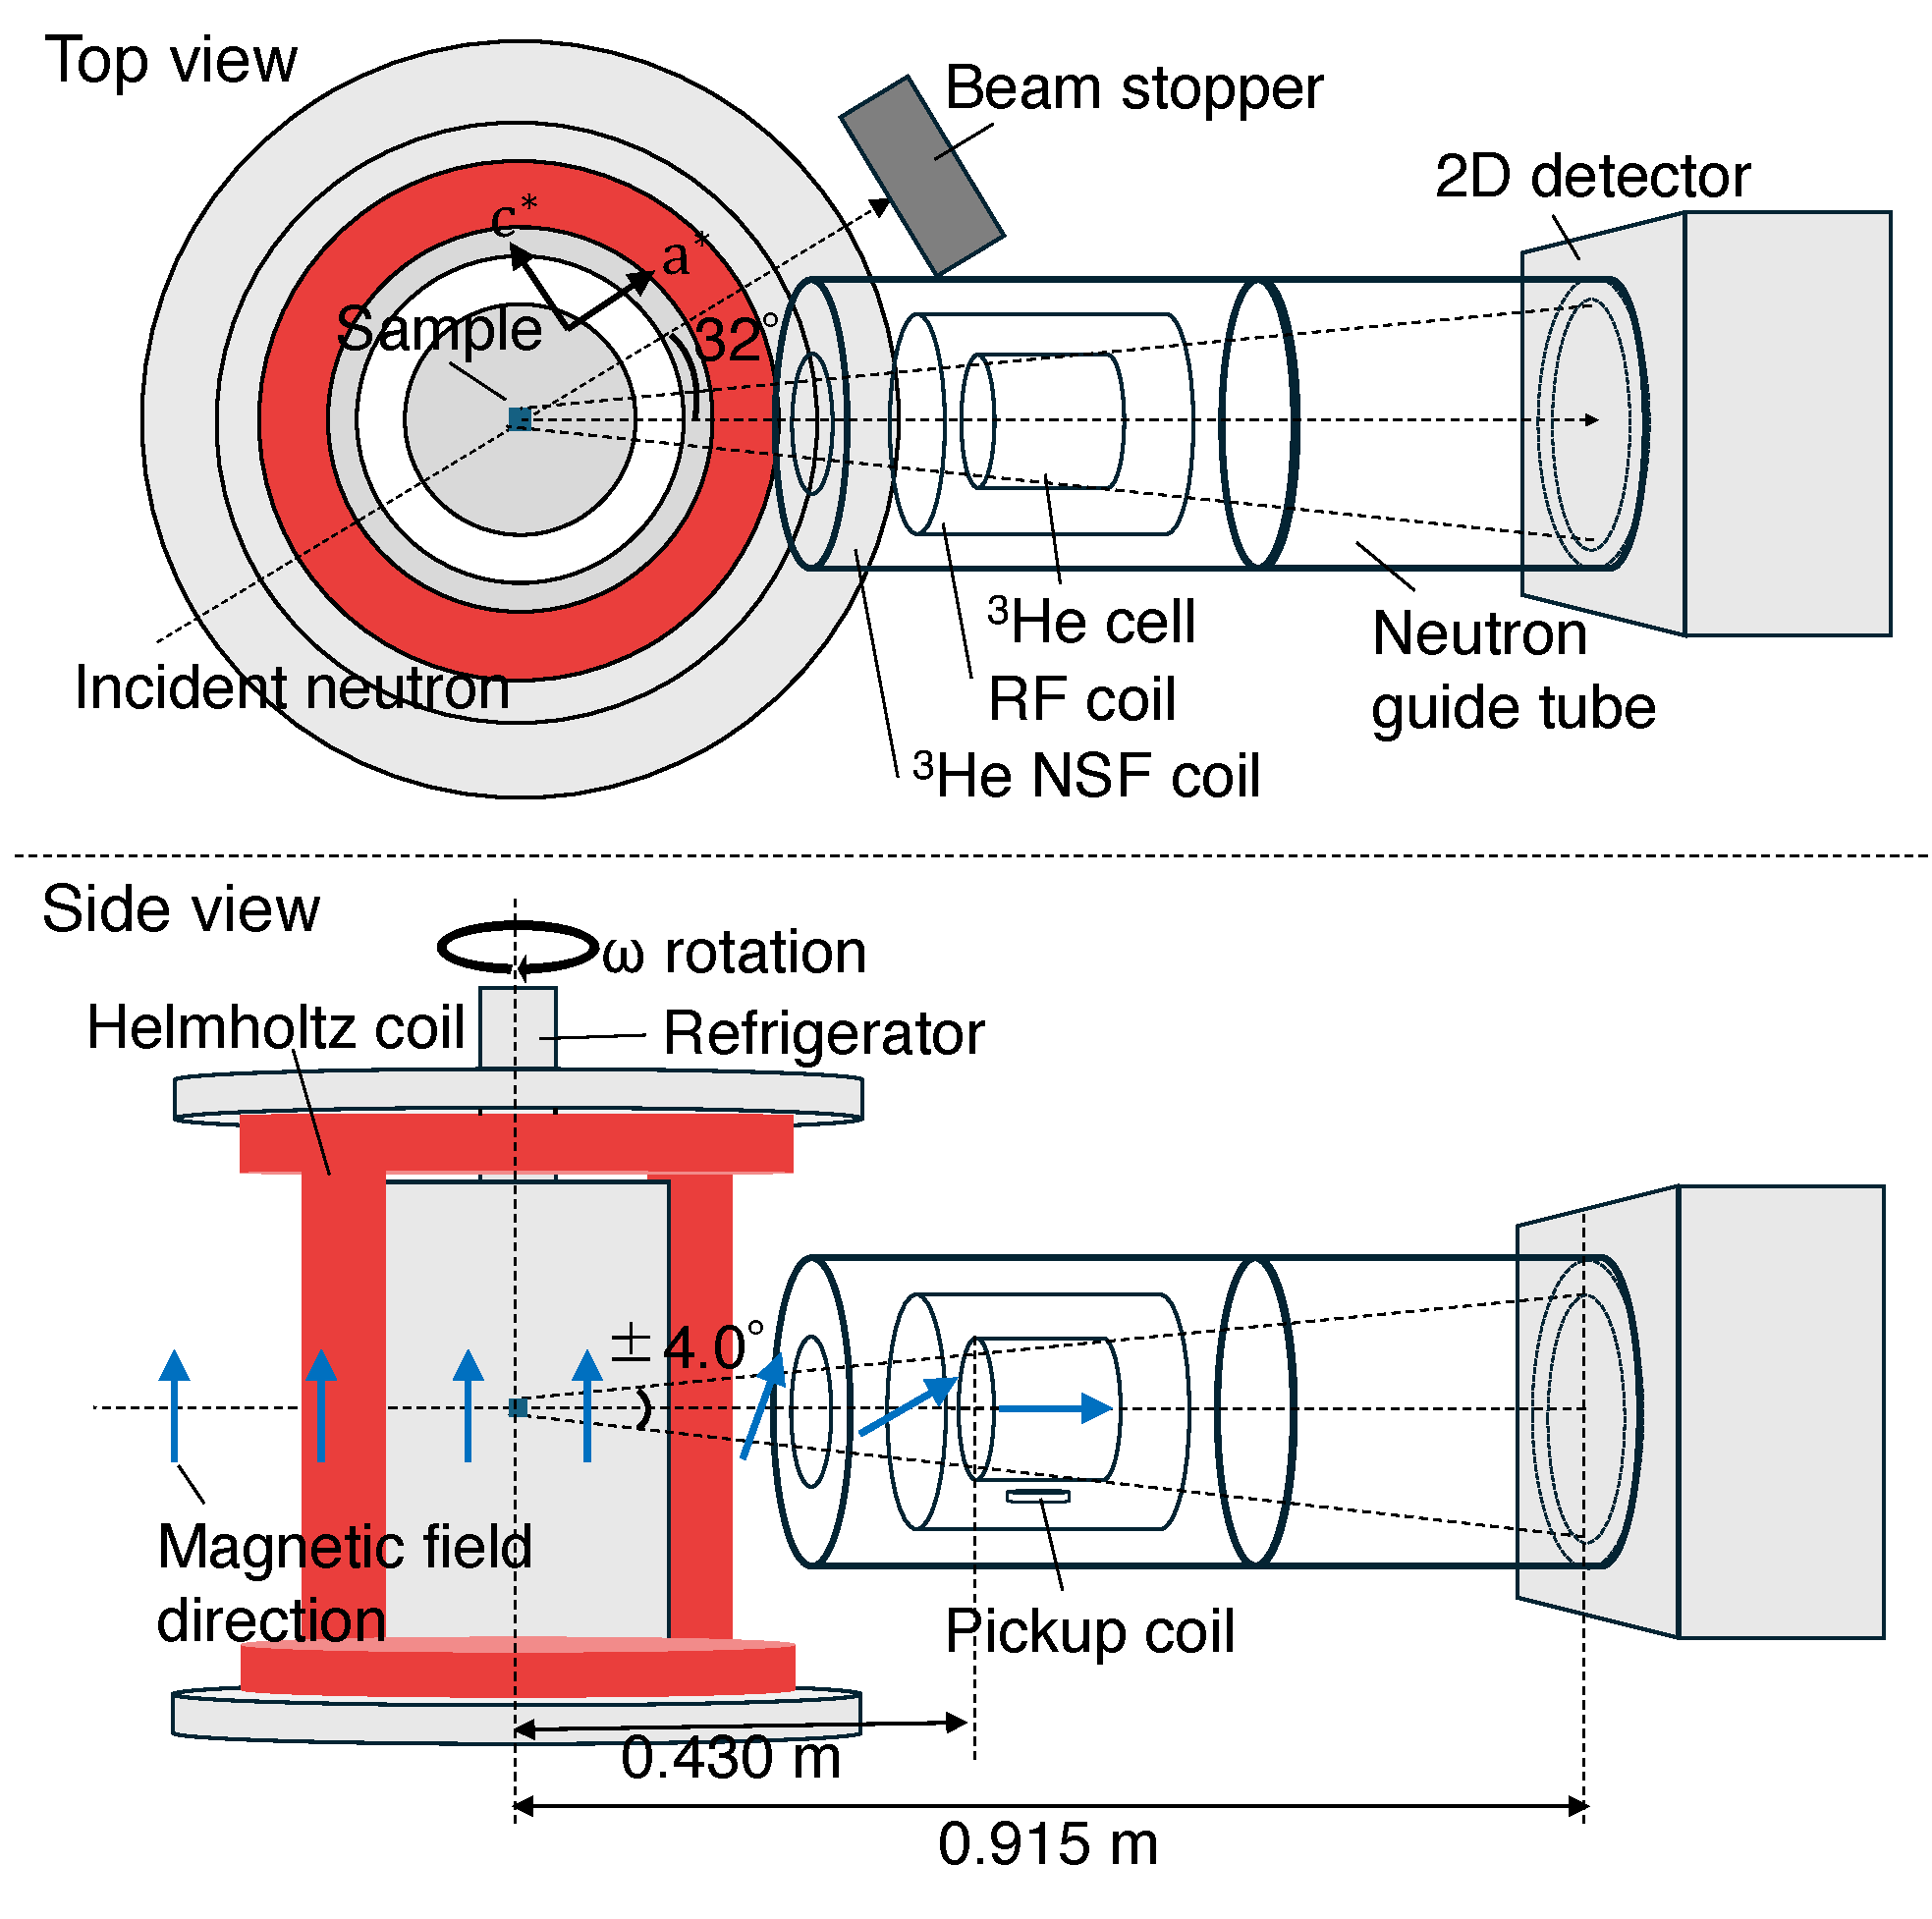
\includegraphics[width=8.5cm]{figure/Scattering_Angle_v7.pdf}
    \DIFaddendFL \caption{
    Schematic illustration of the experimental setup at the 5G PONTA.
    Scattered neutrons from the sample pass through the \Hensf~coil and the neutron guide tube before reaching the 2D detector.
    The sample is mounted in a cryostat that can be rotated by an angle $\omega$.
    The magnetic field direction induced by the Helmholtz coil is vertical, whereas the field within the \Hensf~is oriented along the beam axis.
    The neutron spins are adiabatically rotated to follow the field direction.
    A radiofrequency (RF) coil is used to flip the \He polarization, and an NMR pickup coil monitors the \He polarization after each spin flip.
    }
    \label{fig:Setup}
\end{figure}

\subsection{\He neutron spin filter}
\begin{table*}[t]
\caption{Specifications of \He cells.}
\label{tab:He_cell}
\begin{ruledtabular}
    \begin{tabular*}{\textwidth}{lccccccc}
        Name
        & $D \times L$ (mm)
        & Volume (cm$^3$)
        & \He density (amg)
        & N$_2$ pressure (Torr)
        & K/Rb (mol)\\
        \hline
        Kenji
        & $72 \times 67$
        & 140
        & 3.2
        & 97
        & 26\\
        Shimpachi
        & $72 \times 65$
        & 146
        & 3.1
        & 100
        & 37\\
    \end{tabular*}
\end{ruledtabular}
\end{table*}
The work principle of the \Hensf~is based on the strong spin dependence of the neutron absorption cross section of \He nuclei.
Neutrons with spins antiparallel to the \He nuclear spins are strongly absorbed, while those with spins parallel to the \He nuclear spins are passed through.
Thus, neutrons are polarized by passing through the polarized \He gas.
The two major methods for polarizing \He nuclei are spin-exchange optical pumping (SEOP) \cite{bouchiat_nuclear_1960} and metastability-exchange optical pumping (MEOP).
In the present study, we employed the SEOP method.
In the SEOP method, a glass cell is filled with \He, \ce{N2}, and a small amount of alkali metal.
The cell is irradiated with circularly polarized light resonant with an optical transition of the alkali metal.
The alkali metal electrons undergo repeated excitation and de-excitation, with \ce{N2} serving as a quenching gas to suppress radiative decay, resulting in electron spin polarization.
Then, the polarization of the alkali metal is subsequently transferred to the \He nuclei via spin-exchange collisions, thereby achieving \He nuclear polarization.
The SEOP system used in this study was based on the system developed for the polarized neutron spectrometer POLANO at J-PARC MLF BL23 \cite{ino_development_2017}.
The SEOP system and the polarization analysis coil shown in Fig.~\ref{fig:Setup} are equipped with an adiabatic fast-passage nuclear magnetic resonance (AFP-NMR) system \cite{ino_compact_2012}.
The AFP-NMR system consists of a radio-frequency (RF) coil for flipping the \He polarization and an NMR pickup coil located bottom of the \He cell for monitoring the \He polarization.
Two \He glass cells, named Kenji and Shimpachi, made of aluminosilicate glass (GE180) with nearly identical dimensions were used in this experiment.
Both cells were filled with \He gas, nitrogen gas, and a mixture of alkali-metal atoms (Rb and K) for hybrid SEOP, which provides a hiher pumping efficiency than \ce{Rb}-only SEOP \cite{babcock_hybrid_2003,chen_spin-exchange_2007}.
The details of the cell specifications are described in Table~\ref{tab:He_cell}.
A darkroom to house the SEOP laser system was constructed in the beamline experimental area, where the \He gas was polarized.
After the \He polarization reached saturation, only the \He cell was transported to the \Hensf~coil on the beamline, where neutron measurements were performed during the relaxation of the \He polarization.
This technique is known as the \textit{ex-situ} \Hensf~method.
Since the \He polarization decreases with time in this method, two cells were used alternately for the experiment.
While one cell was used for the polarized neutron experiment, the other was polarized in the SEOP system, and the cells were exchanged every two or three days.



\section{Data reduction procedure including polarization correction}
\begin{figure*}[t]
    \centering
    \DIFdelbeginFL %DIFDELCMD < 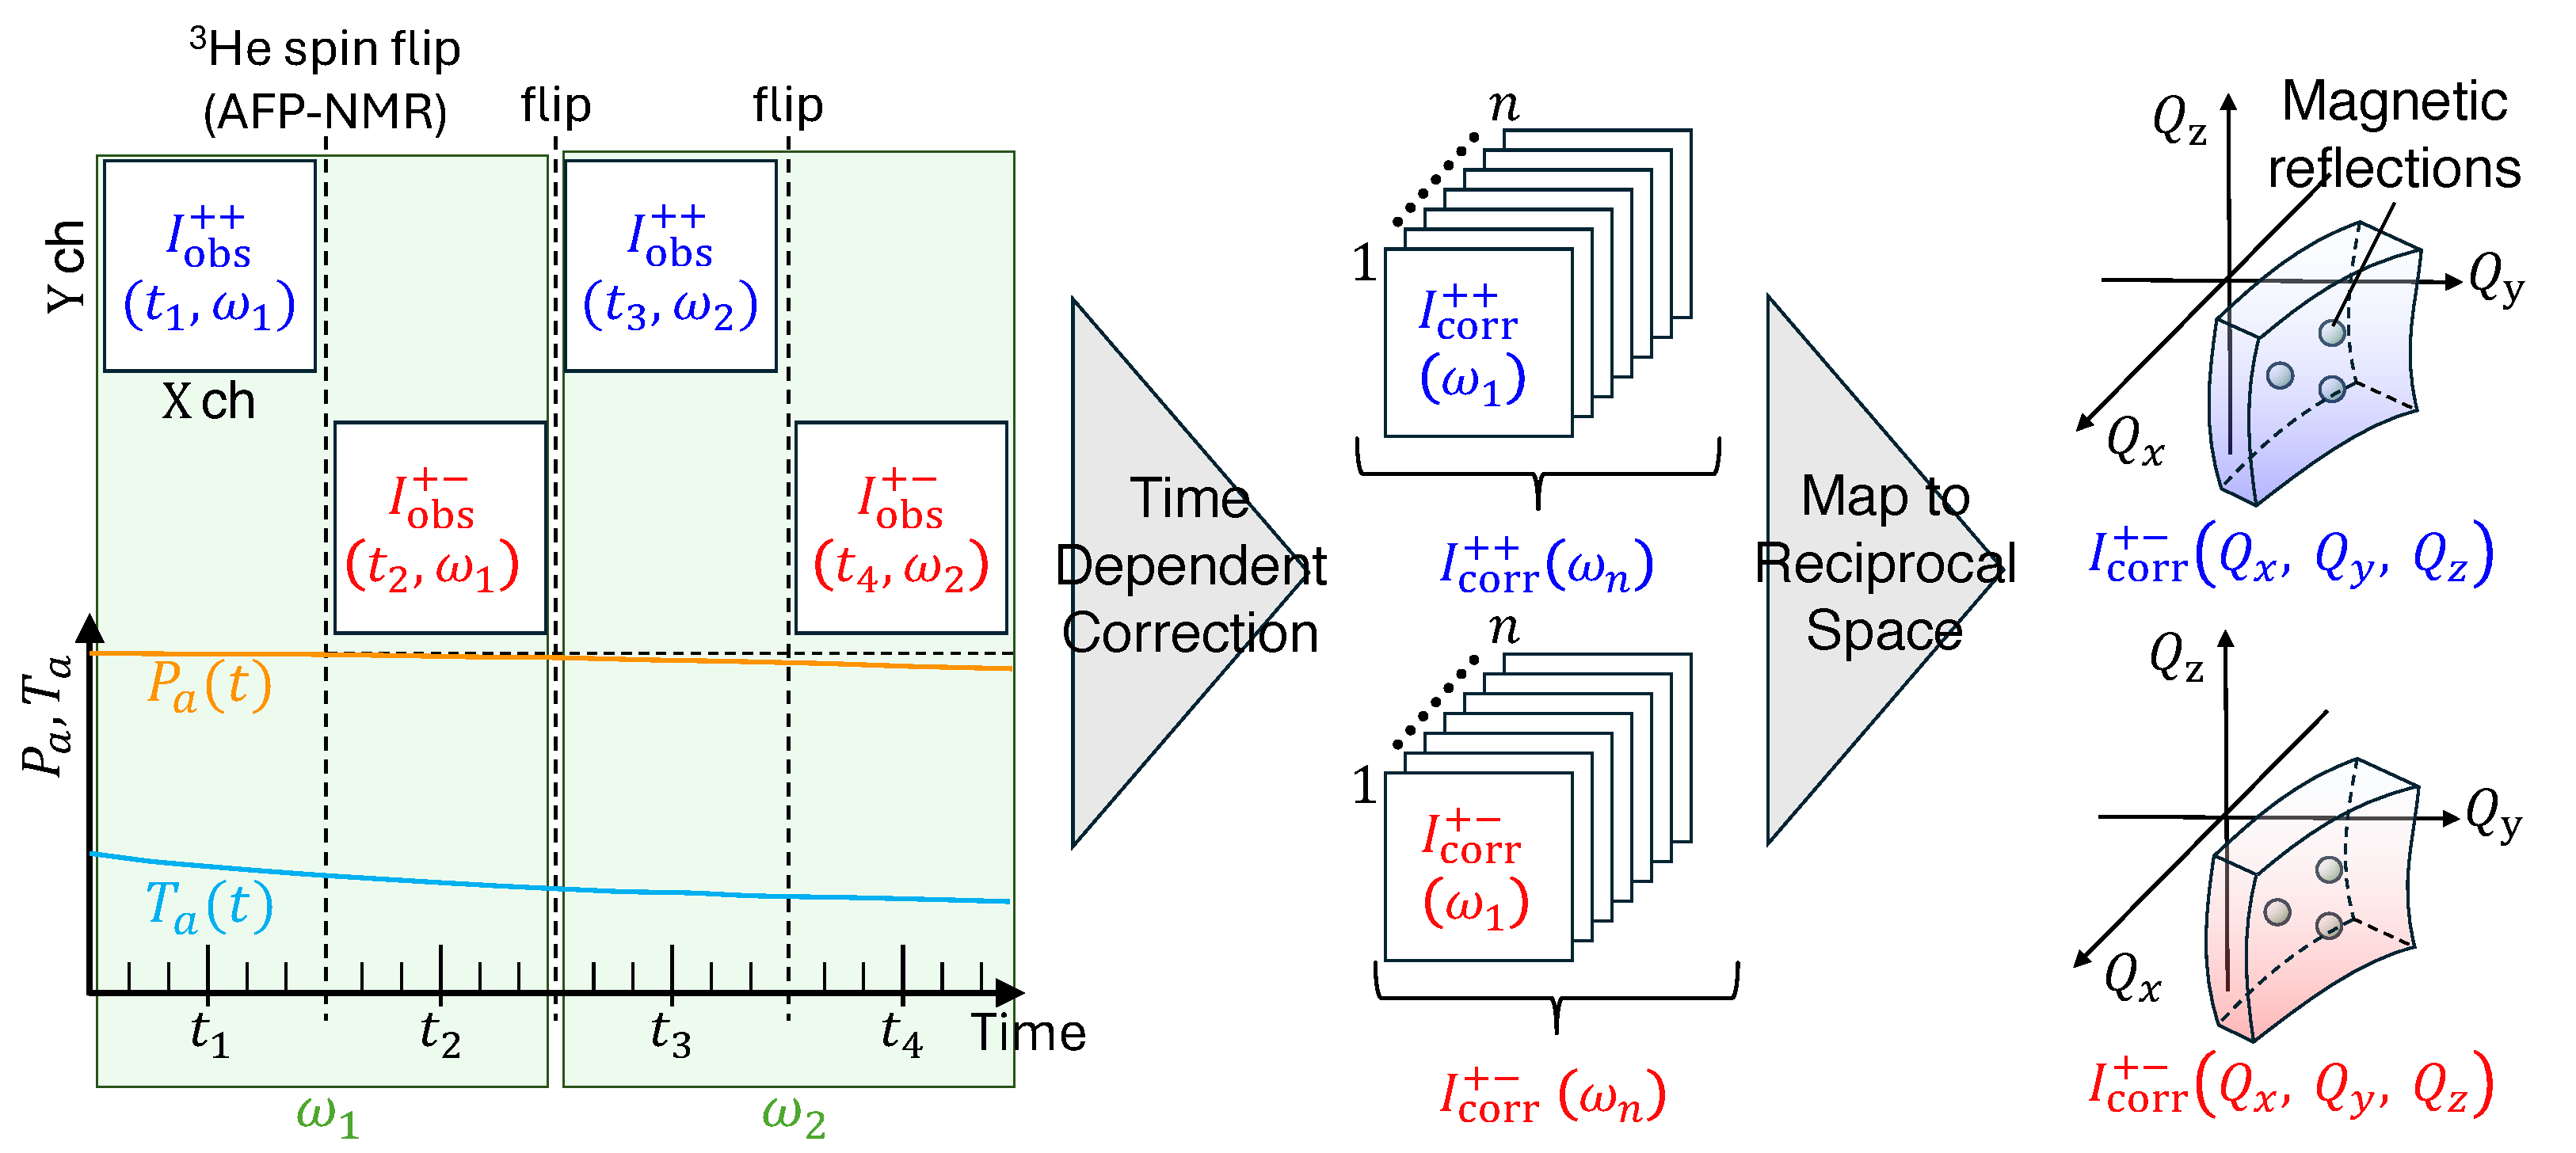
\includegraphics[width=0.8\textwidth]{figure/Procedure_v5.pdf}
%DIFDELCMD <     %%%
\DIFdelendFL \DIFaddbeginFL 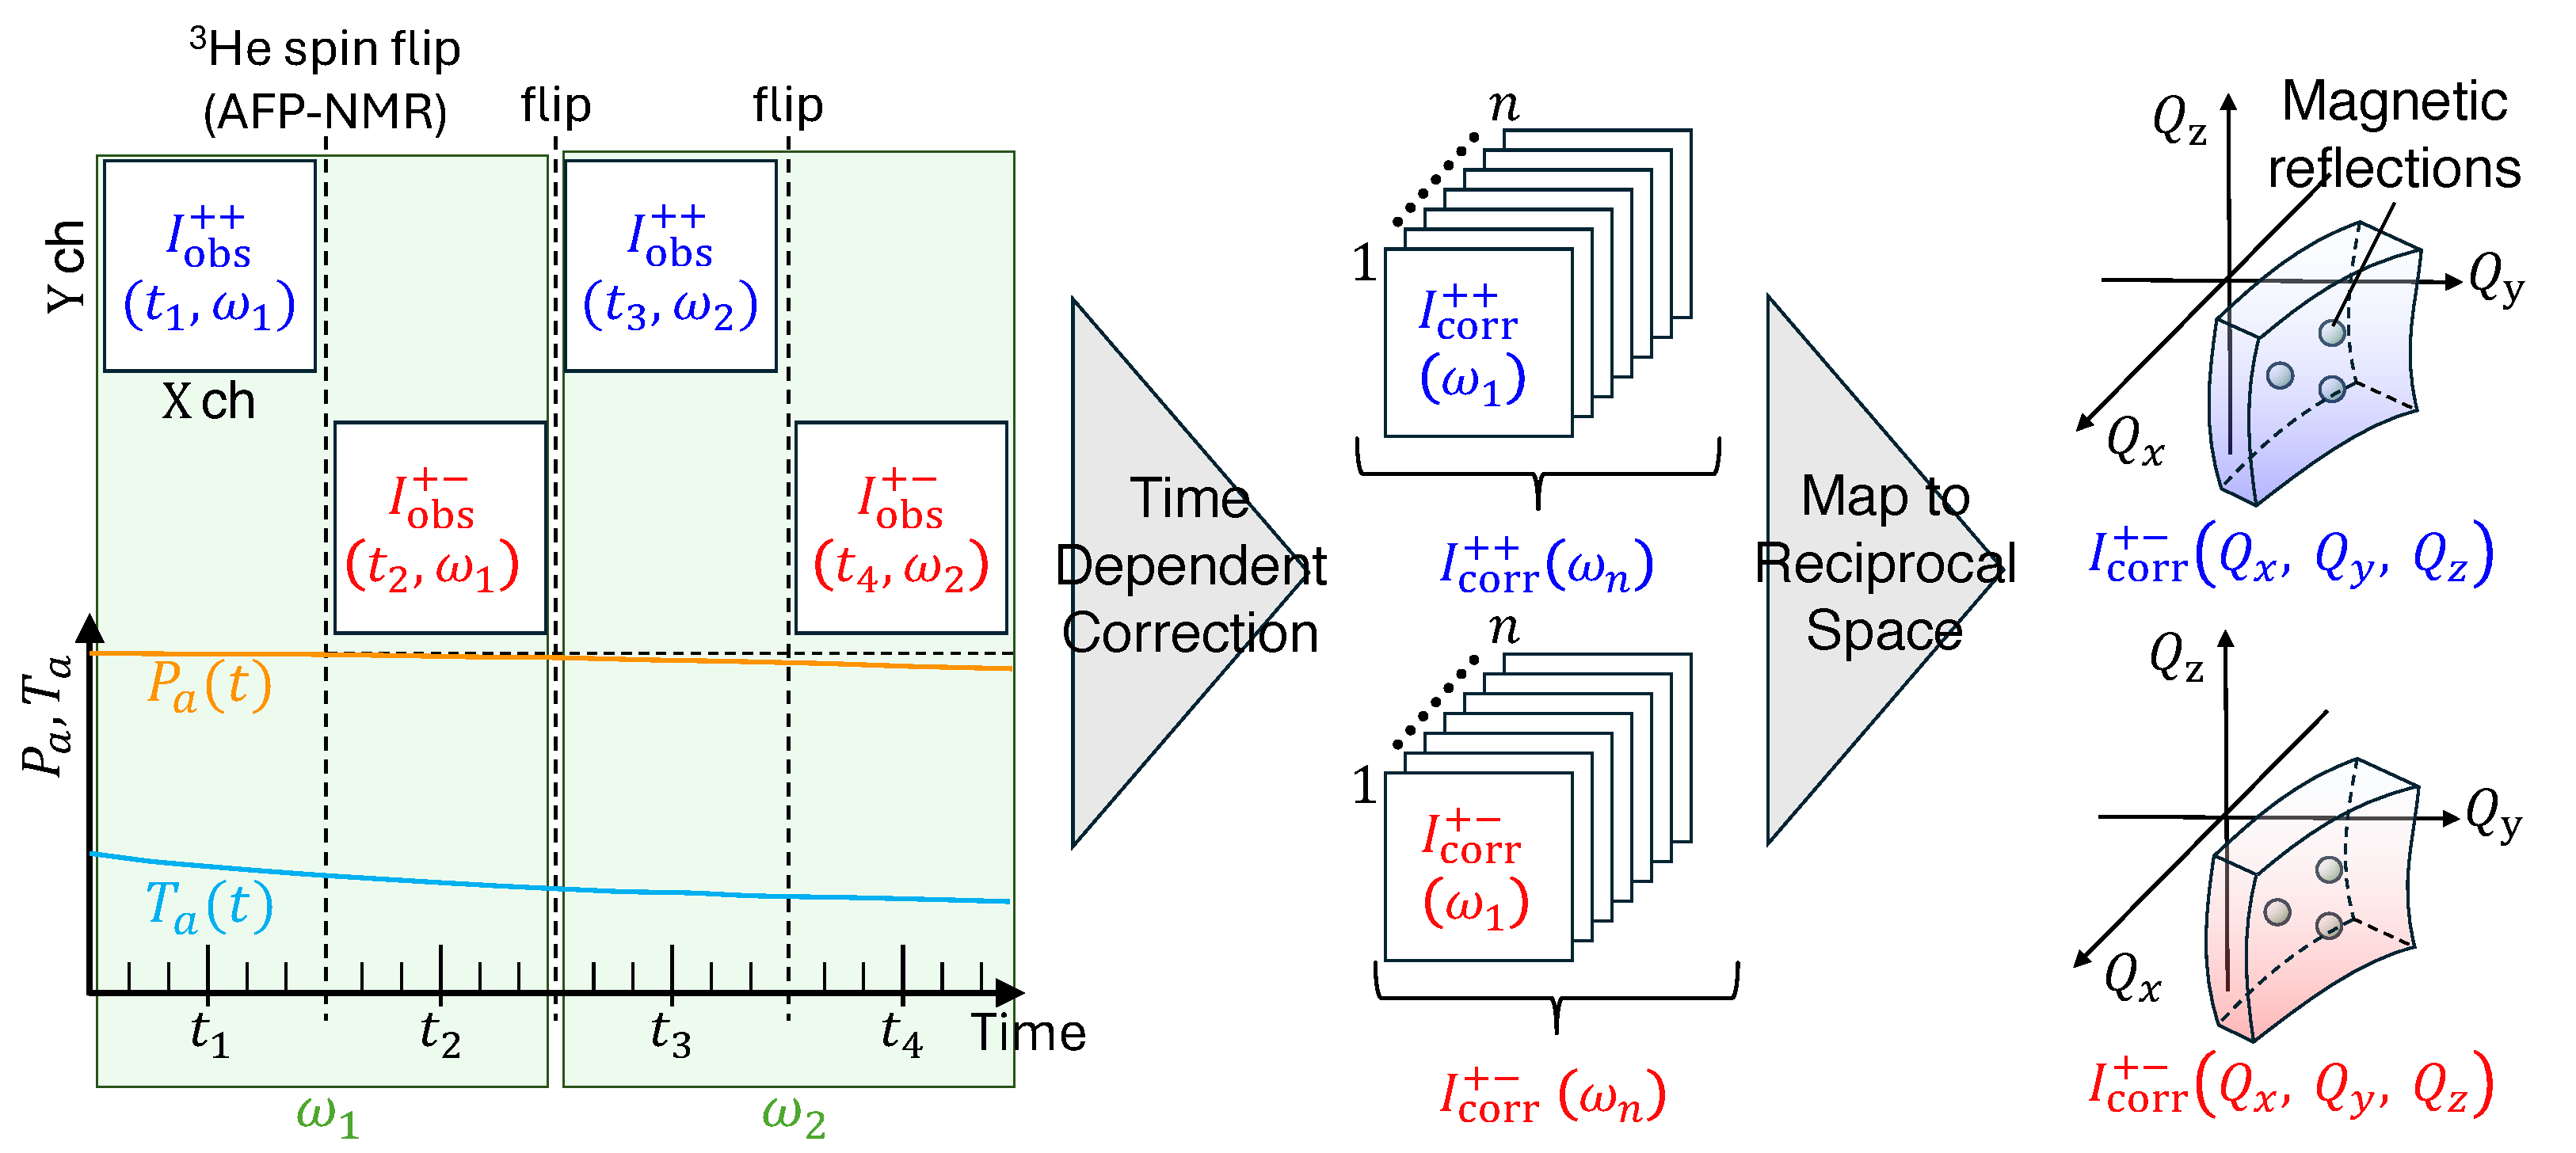
\includegraphics[width=0.8\textwidth]{figure/Procedure_v5.pdf}
    \DIFaddendFL \caption{
    Schematic diagram of the data-reduction procedure for polarization analysis using an \textit{ex-situ} \Hensf~and a 2D detector.
    Raw 2D detector data measured at different sample rotation angles $\omega$ and times $t$ are corrected using the time-dependent neutron polarization $P_n(t_i)$ and transmission $T_n(t_i)$.
    The detector coordinates (X,Y) and sample rotation angle $\omega$ are converted to $Q_x,Q_y,Q_z,$ and then transformed to $H,K,L$ using the UB matrix.
    The corrected three-dimensional reciprocal-space data can then be sliced on an arbitrary plane.
    }
    \label{fig:procedure}
\end{figure*}

% 図と対応させて3stepで話を展開する。
Figure~\ref{fig:procedure} shows the \DIFdelbegin \DIFdel{data acquisition and reduction procedure used to obtain polarization-analysis results for magnetic reflections distributed throughout three-dimensional reciprocal space.
When the }\DIFdelend \DIFaddbegin \DIFadd{procedures of the  data acquisition, reduction and polarization correction in the present study.
At a }\DIFaddend sample rotation angle \DIFdelbegin \DIFdel{was fixed at $\omega= \omega_n$}\DIFdelend \DIFaddbegin \DIFadd{of $\omega=\omega_n$}\DIFaddend , we measured a pair of 2D intensity maps for the non-spin-flip and spin-flip \DIFdelbegin \DIFdel{configurations }\DIFdelend \DIFaddbegin \DIFadd{scatterings }\DIFaddend by flipping the \He polarization.
%DIF >  $t_{2n-1}$ and $t_{2n}$ are the central measurement times for the pair of $I^{++}_\mathrm{obs}$ and $I^{+-}_\mathrm{obs}$, respectively.
\DIFaddbegin \DIFadd{We refer to the observed intensities measured when the polarizations of the neutron and \He nuclei are parallel and antiparallel to each other as $I^{++}_\mathrm{obs}$ and $I^{+-}_\mathrm{obs}$, respectively.
They depend on the position of the detector pixels, the polarizations and transmissions of the polarizer and the analyzer.
Here, we assume that the measurement time of an intensity map is sufficiently shorter than the relaxation time of the \Hensf, and thus the transmission and polarization of \Hensf\ can be approximated to be the values at the midpoint time of the measurement.
}\DIFaddend As shown in Fig.\ref{fig:procedure}, we define the midpoint times of the two successive measurements as $t_{2n-1}$ and $t_{2n}$, respectively.
%DIF <  $t_{2n-1}$ and $t_{2n}$ are the central measurement times for the pair of $I^{++}_\mathrm{obs}$ and $I^{+-}_\mathrm{obs}$, respectively.
\DIFdelbegin \DIFdel{The observed scattering intensities at a detector pixel }\DIFdelend \DIFaddbegin \DIFadd{Thus, the intensities observed at the pixel located at  }\DIFaddend $(x_i, y_j)$ are \DIFdelbegin \DIFdel{expressed }\DIFdelend \DIFaddbegin \DIFadd{described }\DIFaddend as
\begin{widetext}
    \begin{align}
        I^{++}_\mathrm{obs}(\omega_n,t_{2n-1}, x_i,y_j) &= \frac{T_pT_a(t_{2n-1})}{2}\left[\left(1+ P_pP_a(t_{2n-1})\right)I^{++}(\omega_n, x_i,y_j)+\left(1- P_pP_a(t_{2n-1})\right)I^{+-}(\omega_n, x_i,y_j)\right]+\mathrm{BG}(x_i,y_j),
        \label{eq:int_obs_pp}\\
        I^{+-}_\mathrm{obs}(\omega_n,t_{2n}, x_i,y_j) &= \frac{T_pT_a(t_{2n})}{2}\left[\left(1- P_pP_a(t_{2n})\right)I^{++}(\omega_n, x_i,y_j)+\left(1+ P_pP_a(t_{2n})\right)I^{+-}(\omega_n, x_i,y_j)\right]+\mathrm{BG}(x_i,y_j),
        \label{eq:int_obs_pm}
    \end{align}
\end{widetext}
where $I^{++}(\omega_n,x_i,y_j)$ and $I^{+-}(\omega_n,x_i,y_j)$ are the ideal non-spin-flip and spin-flip scattering intensities, respectively.
Here, we assume \DIFaddbegin \DIFadd{that the sample is }\DIFaddend an antiferromagnet in which nuclear and magnetic reflections are separated from each other.
\DIFdelbegin \DIFdel{Under this condition}\DIFdelend \DIFaddbegin \DIFadd{Thus}\DIFaddend , we can impose the conditions of $I^{++} = I^{--}$ and $I^{+-} = I^{-+}$, and \DIFaddbegin \DIFadd{can }\DIFaddend simplify the equations regarding the effect of imperfection of polarization described in Appendix A.
We also note that the chiral magnetic scattering, which depends on the sign of the incident neutron polarization direction, is negrisible because neutron polarization and scattering vector are nearly perpendicular each other \cite{}. %blumeの論文を引っ張ってくる.
$T_p$ and $T_a(t)$ are the neutron transmissions of the Heusler polarizer and \Hensf, respectively.
$P_p$ and $P_a(t)$ are the neutron polarizations of the Heusler polarizer and \Hensf, respectively.
$\mathrm{BG}(x_i,y_j)$ is the background intensity at \DIFdelbegin \DIFdel{detetor pixel }\DIFdelend \DIFaddbegin \DIFadd{the detector pixel of }\DIFaddend $(x_i, y_i)$.
In the present experiment, the background signals were mainly due to imperfect shielding of the \DIFdelbegin \DIFdel{detctor }\DIFdelend \DIFaddbegin \DIFadd{detector }\DIFaddend and neutron flight path.
Thus, we assumed that the background signals are independent of time, \He polarization and the sample rotation angle $\omega$. \DIFdelbegin \DIFdel{We repeated these measurements }\DIFdelend %DIF >
\DIFaddbegin \DIFadd{To measure the background data, we set the $\omega$ angle so as to avoid measuring any Bragg reflections from the sample, and obtained $\mathrm{BG}(x_i,y_j)$.
We repeated the measurements of $I^{++}_\mathrm{obs}$ and $I^{+-}_\mathrm{obs}$ }\DIFaddend with varying the sample rotation angle $\omega$.

\DIFdelbegin \DIFdel{Before converting the data into the intensity distribution in the reciprocal space, we applied the polarization correction to the observed intensity maps taking into account of the relaxation of \He polarization in the }\textit{\DIFdel{ex-situ}}  %DIFAUXCMD
\DIFdel{\Hensf.
}\DIFdelend % In the \textit{ex-situ} \Hensf, both the neutron polarization and transmission decrease with time as the \He polarization relaxes.
% Therefore, the paired intensities $I^{++}_\mathrm{obs}(\omega_n,t_{2n-1})$ and $I^{+-}_\mathrm{obs}(\omega_n,t_{2n})$ are affected differently by the time-dependent polarization and transmission.
\DIFdelbegin \DIFdel{Solving }\DIFdelend \DIFaddbegin \DIFadd{By solving }\DIFaddend Eqs.~\ref{eq:int_obs_pp} and \ref{eq:int_obs_pm} for $I^{++}$ and $I^{+-}$\DIFdelbegin \DIFdel{gives
}\DIFdelend \DIFaddbegin \DIFadd{, we obtain the equations of the polarization correction for the dataset measured at $\omega=\omega_n$ as follows:
}\DIFaddend \begin{widetext}
    \begin{align}
        I^{++}(\omega_n,x_i,y_j) =&
        \frac{1+P_pP_a(t_{2n})}{T_pT_a(t_{2n-1})P_p\left[P_a(t_{2n-1})+P_a(t_{2n})\right]}
        \left[I^{++}_\mathrm{obs}(\omega_n,t_{2n-1},x_i,y_j)-\mathrm{BG}(x_i,y_j)\right]
        \notag\\
        &-
        \frac{1-P_pP_a(t_{2n-1})}{T_pT_a(t_{2n})P_p\left[P_a(t_{2n-1})+P_a(t_{2n})\right]}
        \left[I^{+-}_\mathrm{obs}(\omega_n,t_{2n},x_i,y_j)-\mathrm{BG}(x_i,y_j)\right],
        \\
        I^{+-}(\omega_n,x_i,y_j) =&
        -
        \frac{1-P_pP_a(t_{2n})}{T_pT_a(t_{2n-1})P_p\left[P_a(t_{2n-1})+P_a(t_{2n})\right]}
        \left[I^{++}_\mathrm{obs}(\omega_n,t_{2n-1},x_i,y_j)-\mathrm{BG}(x_i,y_j)\right]
        \notag\\
        &+
        \frac{1+P_pP_a(t_{2n-1})}{T_pT_a(t_{2n})P_p\left[P_a(t_{2n-1})+P_a(t_{2n})\right]}
        \left[I^{+-}_\mathrm{obs}(\omega_n,t_{2n},x_i,y_j)-\mathrm{BG}(x_i,y_j)\right].
        \label{eq:int_corr}
    \end{align}
\end{widetext}
\DIFdelbegin \DIFdel{We applied these corrections to all the pixels using the pairs of 2D intensity maps}\DIFdelend \DIFaddbegin \DIFadd{As we show later, we also experimentally determined the transmissions and polarizations of the polarizer and the analyzer including the temporal decay of the \He polarization.  %DIF >
Substituting all the parameters into the equations above, we corrected the effect of imperfect polarization for all the pixels}\DIFaddend .

% In this way, time-independent scattering intensity data are obtained.
Finally, we convert the detector coordinates and sample rotation angle ($x_i,y_j, \omega_n$) into reciprocal-space coordinates $(Q_x,Q_y,Q_z)$.
% A three-dimensional dataset is then constructed by converting the detector coordinates and sample rotation angle into reciprocal-space coordinates $(Q_x,Q_y,Q_z)$.
The resulting data are further transformed into $(H,K,L)$ coordinates using the UB matrix, allowing the intensity distribution to be sliced along an arbitrary plane in reciprocal space.

%Q空間への転換
% このようにして時間依存しない散乱強度データを得ることができたので、これらを逆空間座標へ転換することで3次元的なデータを得ることできる。
% サンプルの向きと照らし合わせ任意の方向からデータを切り出すことができる。
% After correcting for the time-dependence of the polarization $P_n(t)$ and the transmission $T_n(t)$, the detector coordinates and sample rotation angle were then transformed into reciprocal-space coordinates.
% This transformation allows the polarization-analysis data to be obtained at arbitrary points in reciprocal space.

\section{Results}
\subsection{Evaluation of \He neutron spin filter from nuclear scattering}
\begin{figure}
    \centering
    \DIFdelbeginFL %DIFDELCMD < 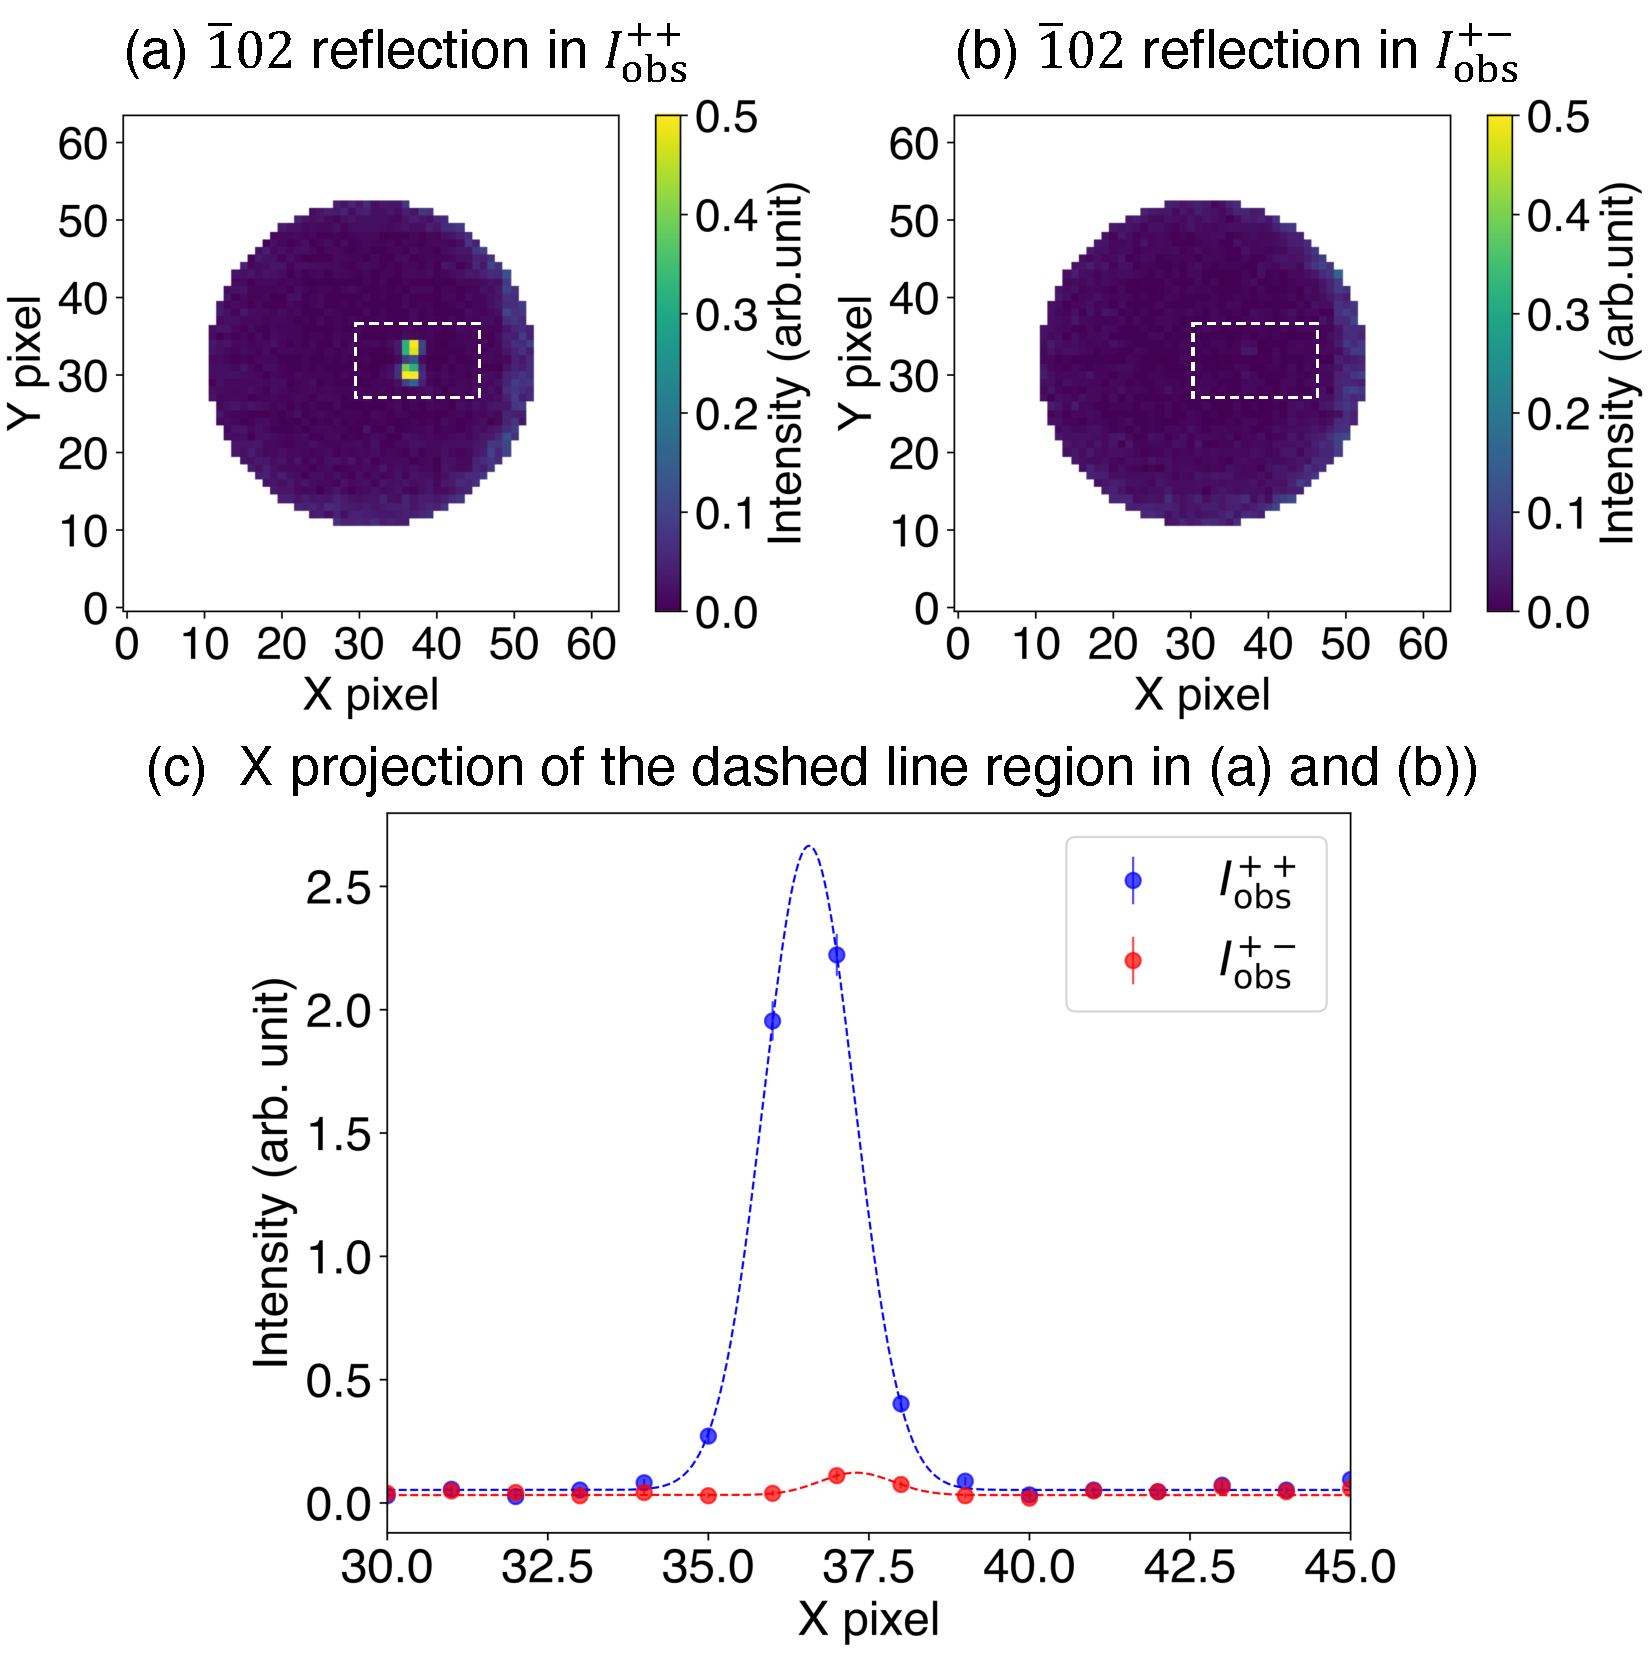
\includegraphics[width=\columnwidth]{figure/raw_data_v9.pdf}
%DIFDELCMD <     %%%
\DIFdelendFL \DIFaddbeginFL 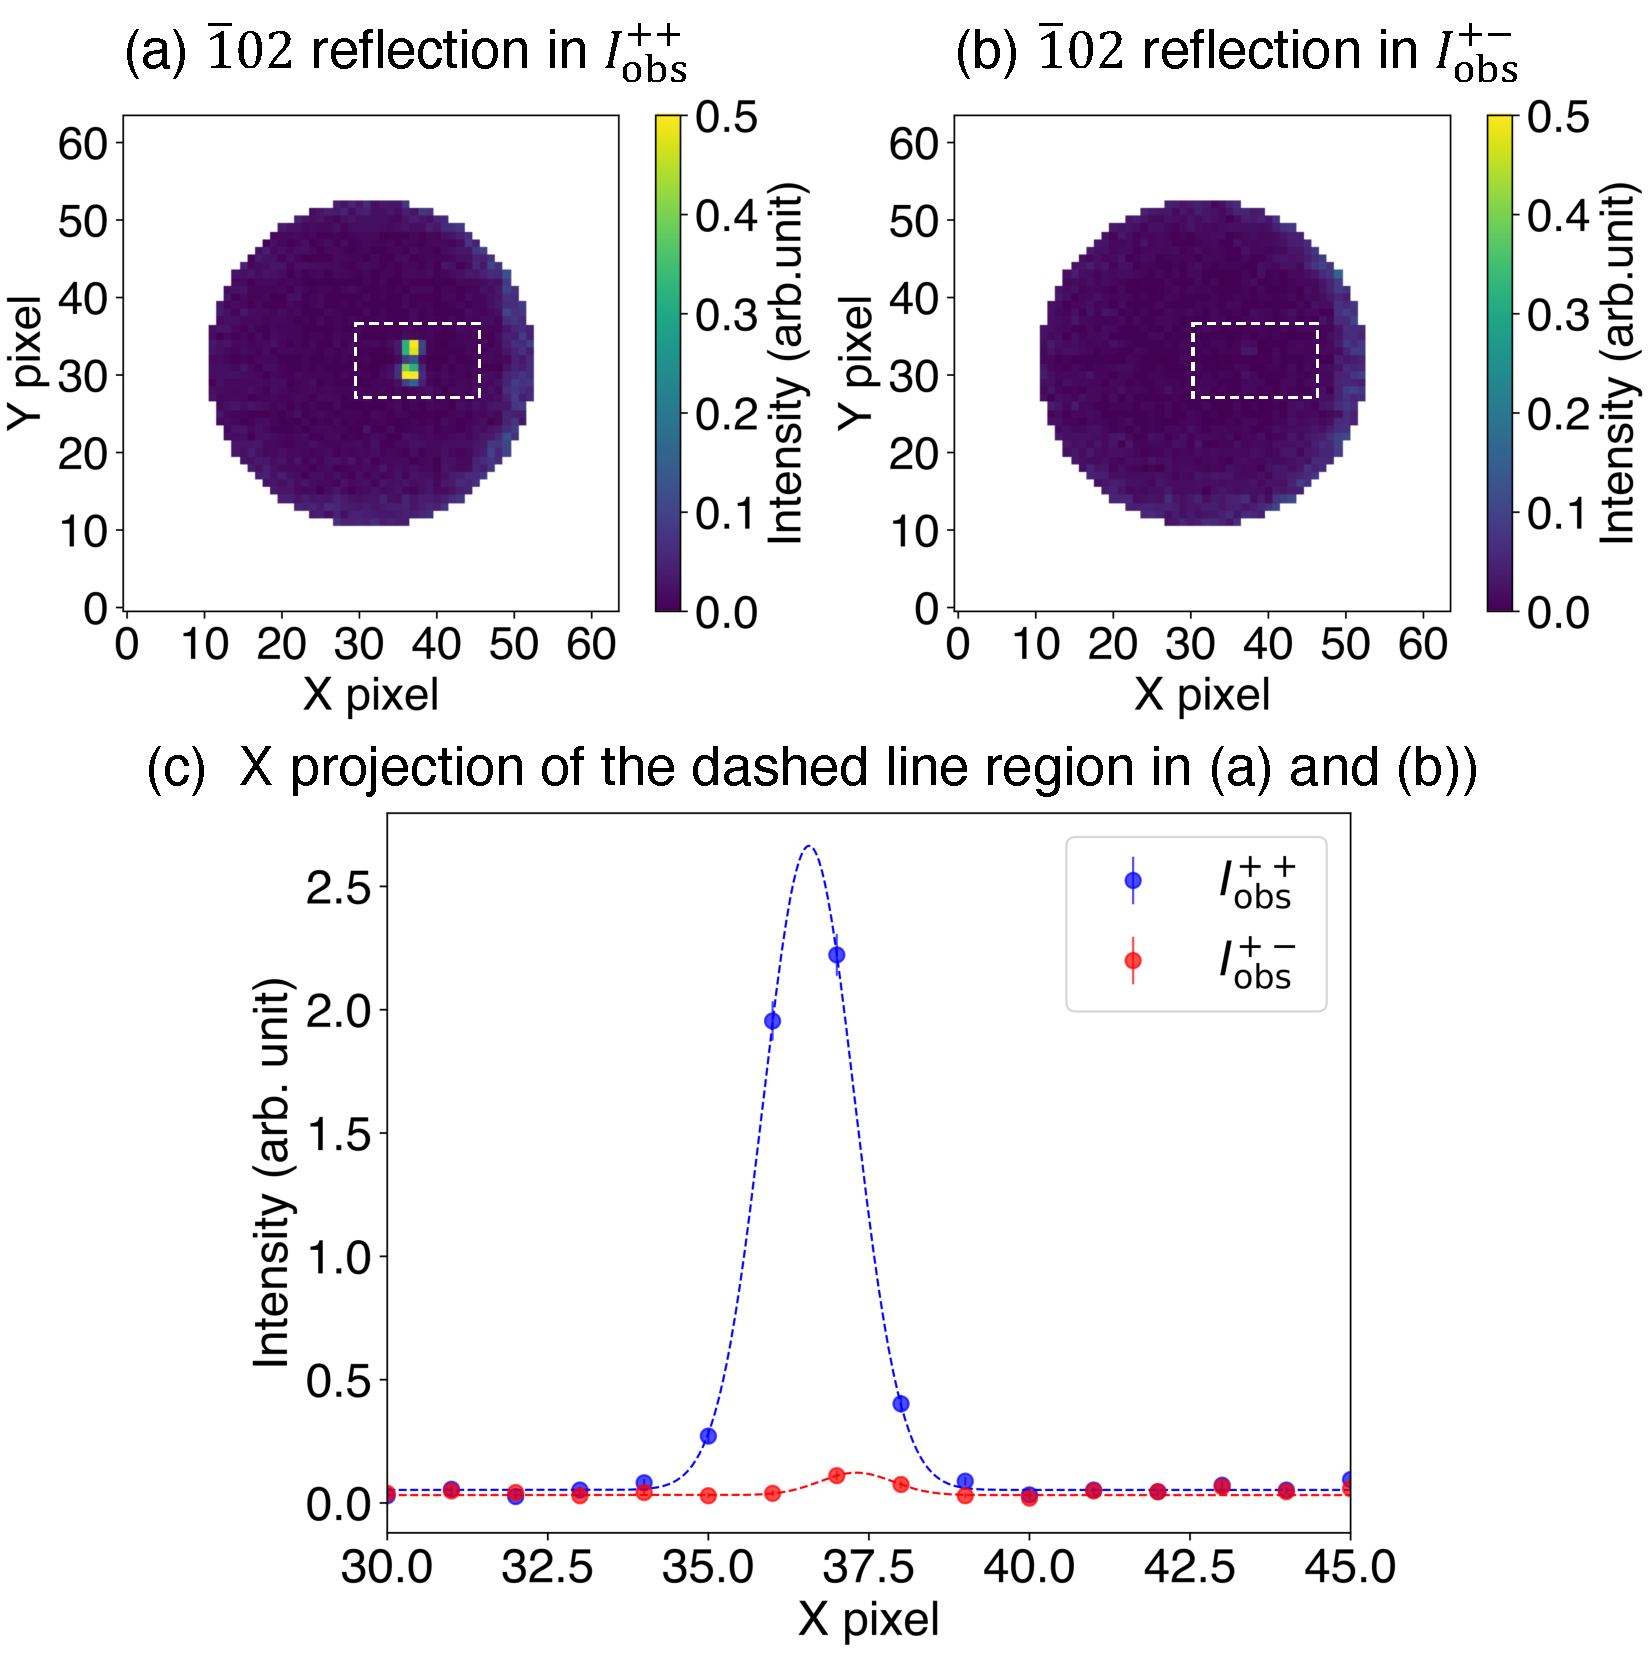
\includegraphics[width=\columnwidth]{figure/raw_data_v9.pdf}
    \DIFaddendFL \caption{(a) Observed non-spin-flip ($I^{++}_\mathrm{obs}$), (b) spin-flip ($I^{+-}_\mathrm{obs}$), and (c) unpolarized ($I^\mathrm{unpol}_\mathrm{obs}$) intensity maps, showing only the analyzing region.
    (d) Line profile along the $x$ direction, obtained by integrating the intensity within the dashed regions in (a), (b), and (c).
    }
    \label{fig:rawdata}
\end{figure}
\begin{figure}
    \centering
    \DIFdelbeginFL %DIFDELCMD < 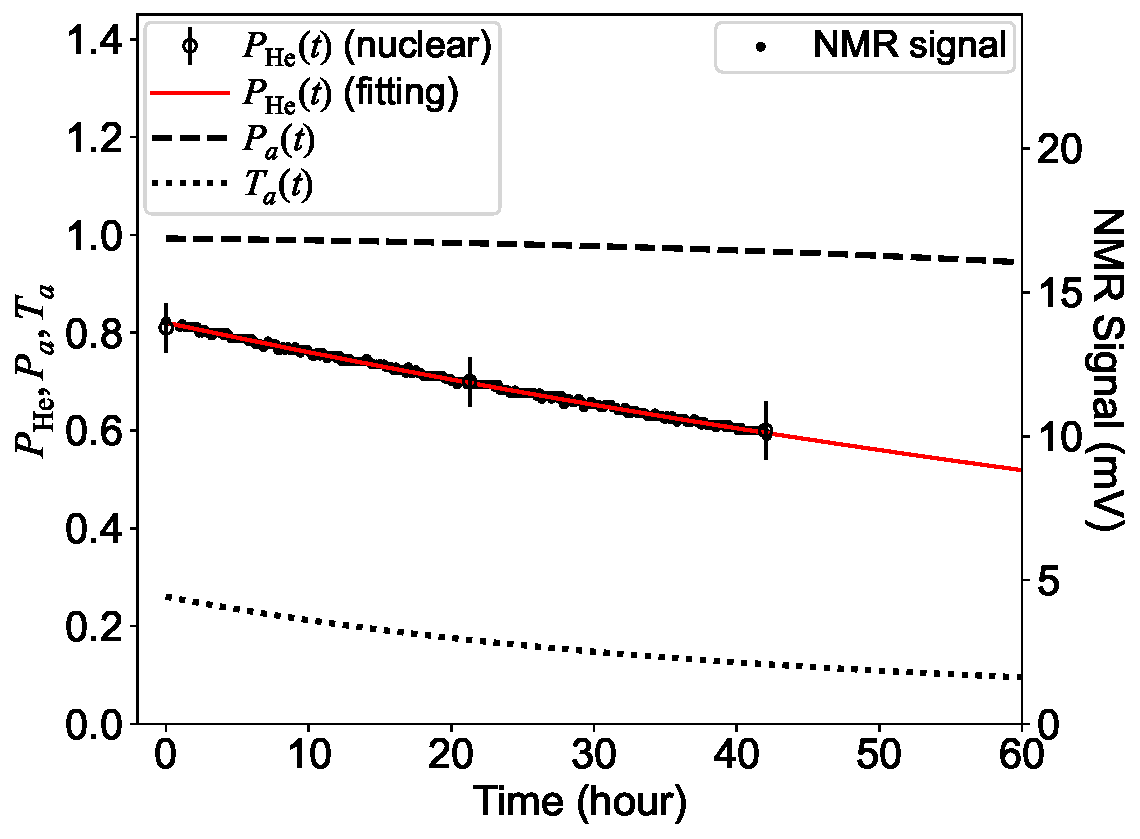
\includegraphics[width=\columnwidth]{figure/NMR_vs_time_20260530.pdf}
%DIFDELCMD <     %%%
\DIFdelendFL \DIFaddbeginFL 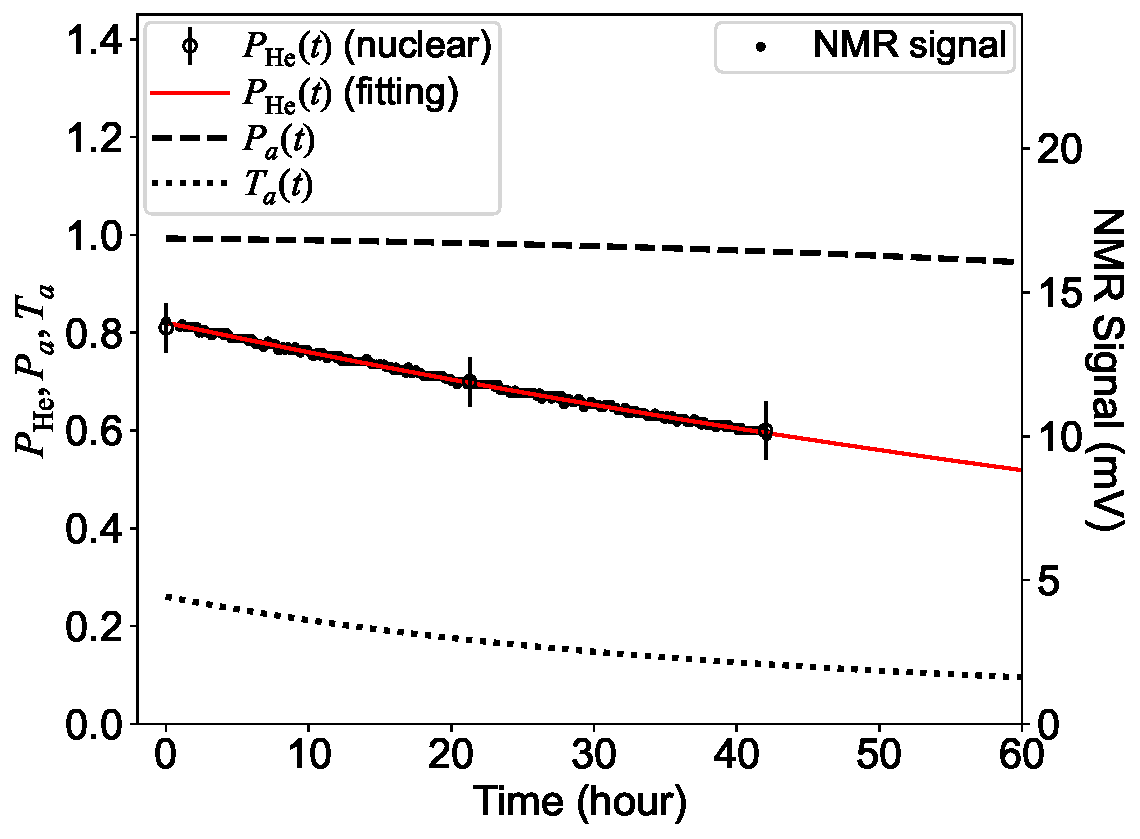
\includegraphics[width=\columnwidth]{figure/NMR_vs_time_20260530.pdf}
    \DIFaddendFL \caption{
        Time dependence of the \He polarization, neutron polarization, and neutron transmission.
        The open circles show the \He polarization determined from the intensity of the $\bar{1}02$ nuclear reflection, while the closed circles show the \He NMR signal.
        The red line represents the fitting result using an exponential decay function.
        The dashed and dot-dashed lines indicate the calculated neutron polarization and transmission, respectively, obtained from the \He polarization.
        }
        \label{fig:pol_trans_decay}
    \end{figure}
    \begin{figure}
        \centering
        \DIFdelbeginFL %DIFDELCMD < 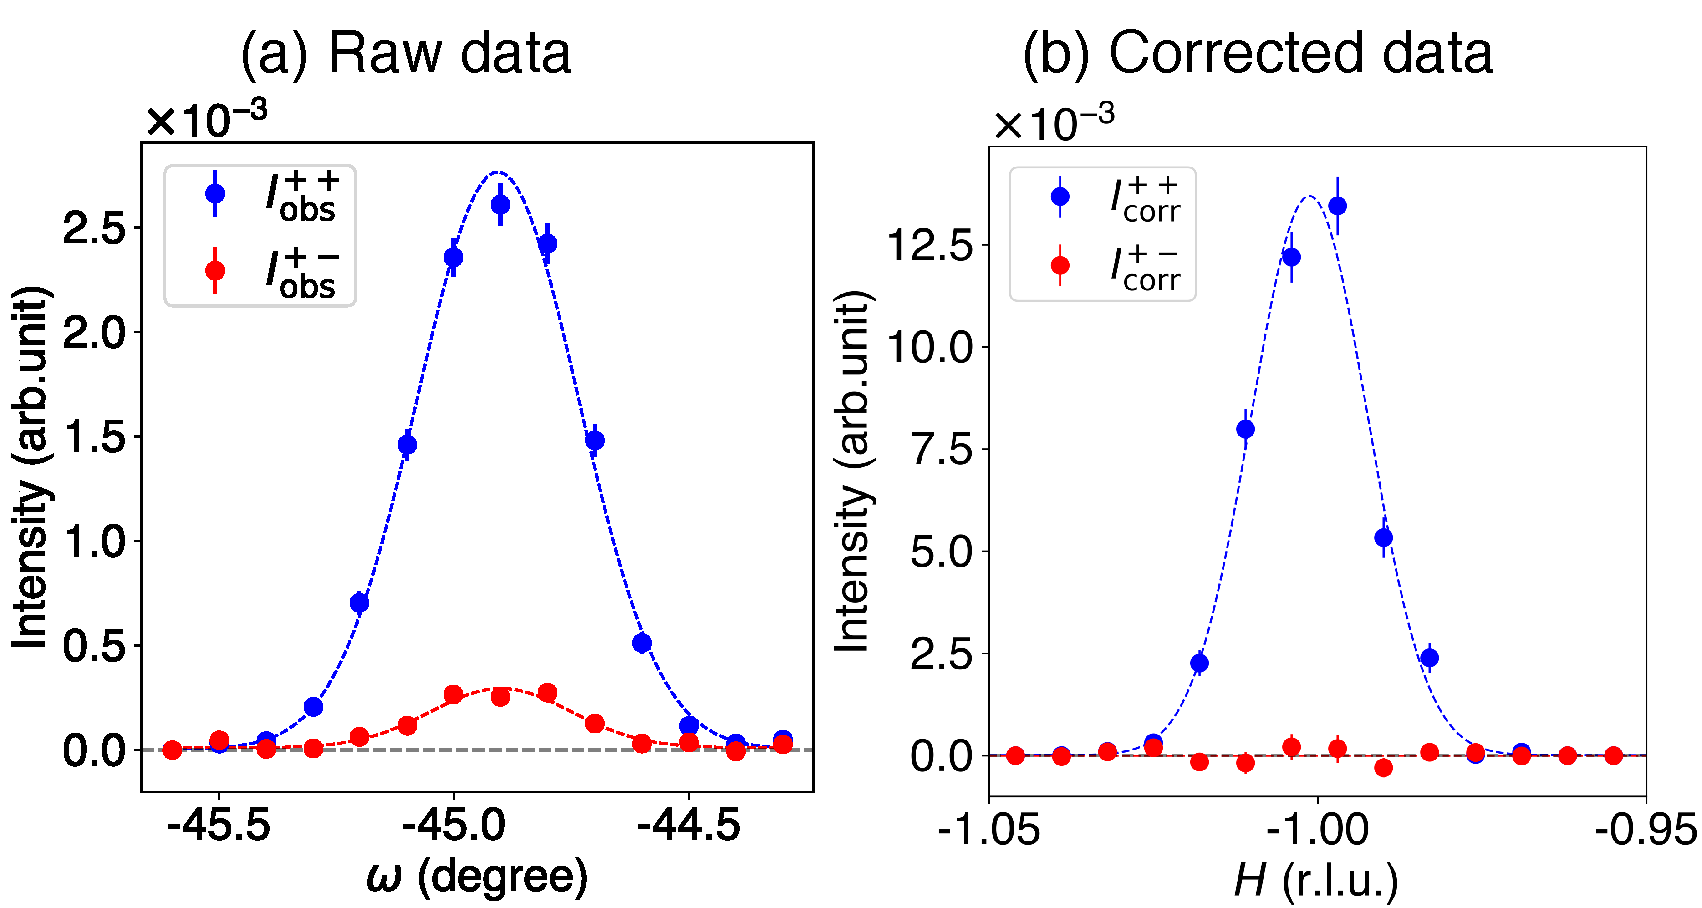
\includegraphics[width=\columnwidth]{figure/Polarization_correction_v6.pdf}
%DIFDELCMD <         %%%
\DIFdelendFL \DIFaddbeginFL 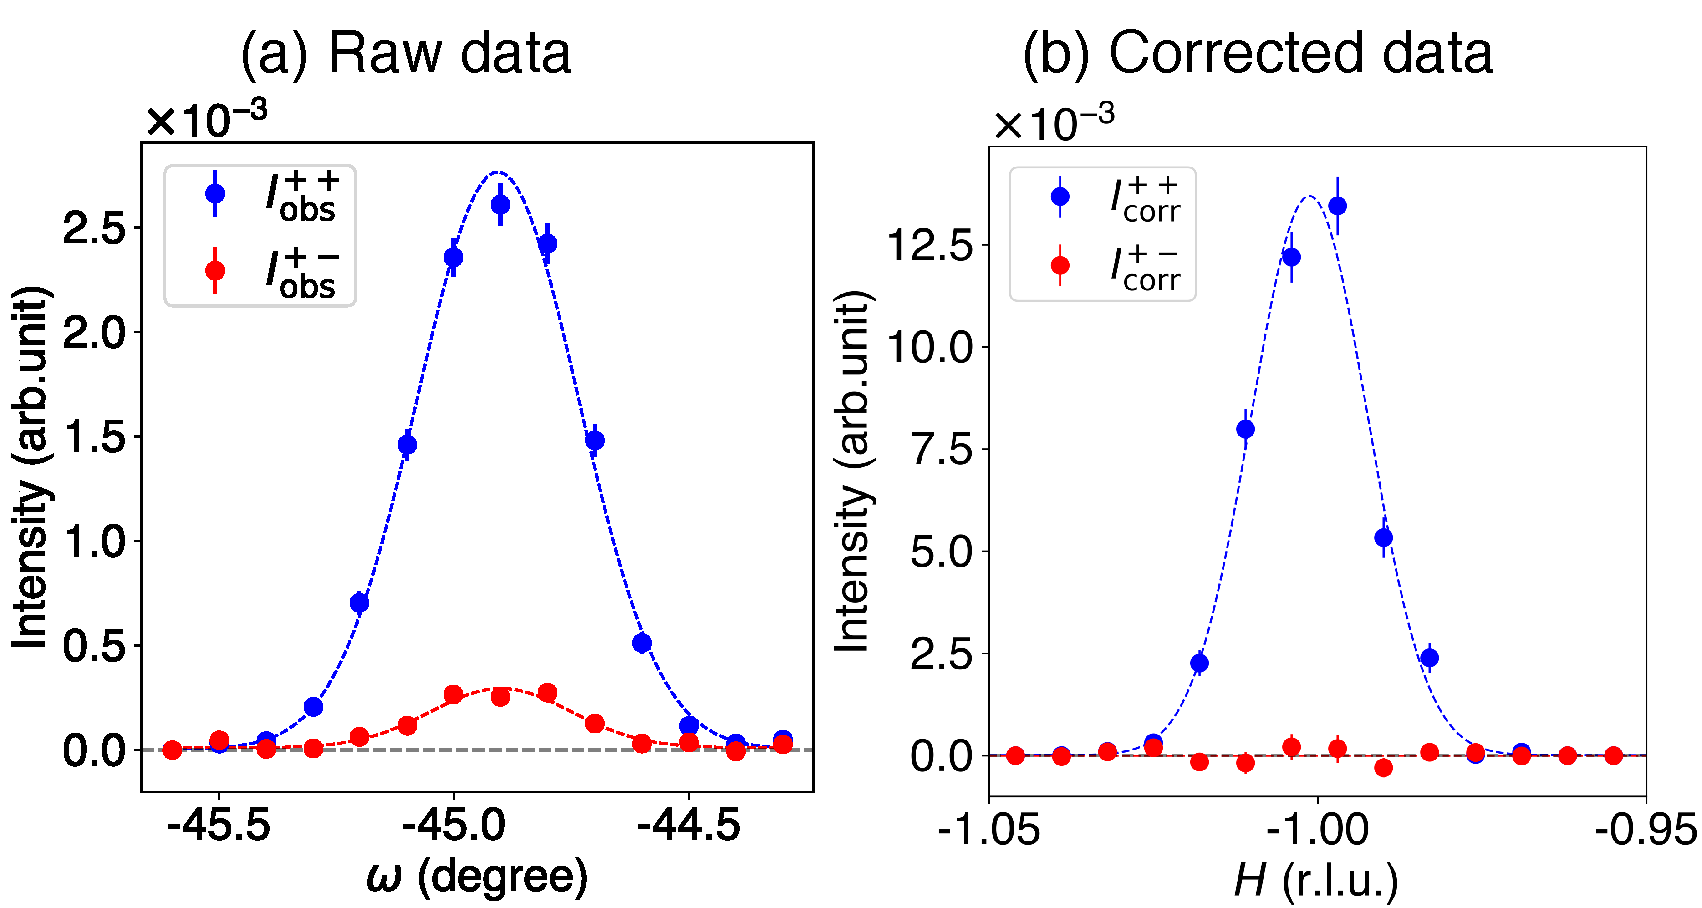
\includegraphics[width=\columnwidth]{figure/Polarization_correction_v6.pdf}
        \DIFaddendFL \caption{The measured intensity of the $\bar{1}02$ reflection integrated over the peak region identified on the 2D detector while scanning the sample rotation angle $\omega$.
        (a) Raw data, where the red and blue symbols represent the non-spin-flip intensity $I^{++}_\mathrm{obs}$ and spin-flip intensity $I^{+-}_\mathrm{obs}$, respectively.
        (b) Corrected data, where the red and blue symbols represent the corrected non-spin-flip and spin-flip scattering cross sections, $\Sigma^{++}_\mathrm{obs}$ and $\Sigma^{+-}_\mathrm{obs}$, respectively.}
        \label{fig:polcorrection}
    \end{figure}

    \label{sec:He-3}
    % 3He 偏極度の時間依存性を調べるために核反射による見積もりを行った。
    \DIFaddbegin \DIFadd{The }\DIFaddend \He polarization is usually evaluated by measuring the transmission of a neutron beam through the \He cell.
    However, the \He \DIFdelbegin \DIFdel{cell cannot }\DIFdelend \DIFaddbegin \DIFadd{could not }\DIFaddend be placed in the \DIFdelbegin \DIFdel{direct }\DIFdelend path of the \DIFaddbegin \DIFadd{incident }\DIFaddend neutron beam in \DIFdelbegin \DIFdel{this experiment because of the detector's sensitivity}\DIFdelend \DIFaddbegin \DIFadd{the present experimental setup}\DIFaddend .
    Therefore, the \He polarization was evaluated \DIFdelbegin \DIFdel{from the }\DIFdelend \DIFaddbegin \DIFadd{by measuring a }\DIFaddend nuclear Bragg peak\DIFdelbegin \DIFdel{intensity. }\DIFdelend \DIFaddbegin \DIFadd{. %DIF >
    Specifically, we selected the $\bar{1}02$ reflection, which has a similar scattering angle to that of the magnetic reflections of interest.
    }\DIFaddend The neutron transmission $T_a(t)$, the neutron polarization $P_a(t)$, and the \He polarization $P_\mathrm{He}(t)$ are given by the following equations \cite{coulter_neutron_1990}:
    \begin{align}
        T_a(t) &= T_\mathrm{cell}\exp(-\mathcal{O}(\lambda))\cosh(\mathcal{O}(\lambda)P_\mathrm{He}(t)),
        \label{eq:transmission_3He}\\
        P_a(t) &= \tanh(\mathcal{O}(\lambda)P_\mathrm{He}(t)),
        \label{eq:pol_n3He}\\
        P_\mathrm{He}(t) &= P_\mathrm{He,0} \exp(-t/\tau),
        \label{eq:pol_3He}
    \end{align}
    Here, $T_\mathrm{cell}$ is the transmission of the \He glass cell.
    $\mathcal{O}$ is the opacity of \He cell, defined as $\mathcal{O} = \rho d \sigma$.
    $\rho$ is the number density of \He, and $d$ is the \He gas thickness.
    $\sigma(\lambda)$ is the neutron absorption cross section of unpolarized \He.
    $P_{\mathrm{He},0}$ is the initial polarization at $t=0$, and $\tau$ is the relaxation time.
    According to the literature, the $\sigma(\lambda)$ at $\lambda = 2.36\ \textrm{\AA}$ is $6992~\textrm{barn}$ \cite{passell_measurement_1966}.

    First, the gas thickness $\rho d$ of each cell was determined \DIFdelbegin \DIFdel{by measuring a nuclear Bragg reflection.
    In the present measurement, we selected the $\bar{1}02$ reflection which has a simillar scattering angle to that of the magnetic reflections of interest.
    }\DIFdelend \DIFaddbegin \DIFadd{as follows.
    }\DIFaddend % I^{unpol}の測定でやったことを記述する。
    Before polarizing \He by SEOP, we measured the nuclear peak \DIFdelbegin \DIFdel{at $\omega$ which satisfy the Bragg condition }\DIFdelend through the unpolarized \He cell \DIFaddbegin \DIFadd{while fixing $\omega$ at the Bragg condition}\DIFaddend .
    From the intensity map, we extracted a box-integrated intensity near the peak.
    \DIFdelbegin \DIFdel{By subtlacting the baclground signalsestimated from the intensities in the surrounding the pixels}\DIFdelend \DIFaddbegin \DIFadd{After subtracting the background signals}\DIFaddend , we obtained the integrated intensity of the Bragg reflection, $\mathcal{I}_\mathrm{obs}^\mathrm{unpol}$.
    By using eqs \ref{eq:int_obs_pp}, \ref{eq:transmission_3He}, \ref{eq:pol_3He} and $P_\mathrm{He}=0$, $\mathcal{I}_\mathrm{obs}^\mathrm{unpol}$ is expressed as follows.
    \begin{equation}
        \mathcal{I}^\mathrm{unpol}_\mathrm{obs}
        =\sum_{(i,j)\in R}
        \left(
        \frac{T_p}{2}
        T_\mathrm{cell}
        \exp[-\mathcal{O}(\lambda)]
        I^{++}(x_i,y_j)
        % +\mathrm{BG}(x_i,y_j)
        \right).
    \end{equation}
    where $R$ denotes the box-integrated region.
    Note that the nuclear Bragg reflection contains only the non-spin-flip scattering intensity, and thus \DIFaddbegin \DIFadd{we can impose }\DIFaddend $I^{+-} = 0$ \DIFdelbegin \DIFdel{.
    }\DIFdelend \DIFaddbegin \DIFadd{in Eq. (\ref{eq:int_obs_pp}).
    }\DIFaddend % The transmission through the unpolarized \He cell, $T_\mathrm{cell}\exp[-\mathcal{O}(\lambda)]$, is obtained from Eq.~\ref{eq:transmission_3He} by setting $P_\mathrm{He}=0$.
    The same measurement was performed using an empty cell with the same dimensions as the \He glass cell to obtain $\mathcal{I}^\mathrm{empty}_\mathrm{obs}$, where the transmission term $T_\mathrm{cell}\exp[-\mathcal{O}(\lambda)]$ is replaced by $T_\mathrm{cell}$.
    Then, taking the ratio $\mathcal{I}^\mathrm{unpol}_\mathrm{obs}/\mathcal{I}^\mathrm{empty}_\mathrm{obs}$\DIFdelbegin \DIFdel{allows the gas thickness $\rho d$ to be determined.
    %DIF <  Note that the background intensity $\mathrm{BG}(x_i,y_j)$ was estimated from the data at sample rotation angles away from the Bragg condition.
    As a result}\DIFdelend ,  the $\rho d$ values of the Kenji and Shimpachi cells were determined to be $18.5 \pm 0.5~\mathrm{amg\,cm}$ and $18.8 \pm 0.4~\mathrm{amg\,cm}$, respectively.
%DIF <  ↑もうちょっと簡略化させて一文で書けるかも。

    % The summation is taken over the rectangular peak region on the detector.
    % Since an empty cell has zero opacity, the ratio of the nuclear Bragg intensities measured with the \He cell and the empty cell is given by $\exp(-\rho d \sigma(\lambda))$.
    % As a result, the $\rho d$ of Kenji cell and Shimpachi cell were deterimined by $18.5 \pm 0.5\ \textrm{amg cm}$ and $18.8 \pm 0.4\ \textrm{amg cm}$, respectively.

    Second, \DIFaddbegin \DIFadd{we determined $P_\mathrm{He,0}$ in Eq. (\ref{eq:pol_3He}) by measuring the nuclear reflection with the polarized \He cell.
    Immediately after }\DIFaddend the \DIFdelbegin \DIFdel{$P_\mathrm{He}(t)$ was determined .
    After polarizing the }\DIFdelend \He \DIFdelbegin \DIFdel{by SEOP, the \He }\DIFdelend cell was \DIFdelbegin \DIFdel{transported }\DIFdelend \DIFaddbegin \DIFadd{moved from the SEOP system }\DIFaddend to the beamline, \DIFdelbegin \DIFdel{and then the $I^{++}_\mathrm{obs}$ }\DIFdelend \DIFaddbegin \DIFadd{we obtained the integrated intensities of the reflection when the \He polarization is parallel and antiparallel to the incident neutron polarization, which are referred to as $\mathcal{I}^\mathrm{++}_\mathrm{obs}(t=0)$ }\DIFaddend and \DIFdelbegin \DIFdel{$I^{+-}_\mathrm{obs}$ of the nuclear reflection were measured}\DIFdelend \DIFaddbegin \DIFadd{$\mathcal{I}^\mathrm{+-}_\mathrm{obs}(t=0)$, respectively, in the same manner as the measurement with the unpolarized \He cell}\DIFaddend .
    As shown in Fig.~\ref{fig:rawdata}, we clearly observed the nuclear Bragg peak in the non-spin flip channel\DIFaddbegin \DIFadd{, while the intensity in the spin-flip channel was extremely weak}\DIFaddend .
    Note that the peak in Fig.~\ref{fig:rawdata}(a) shows the tiny splitting because of the mosaicity of the single crystal sample.
    \DIFdelbegin \DIFdel{Here, we defined the time origin ($t=0$) as the center of the measurement times of $I^{++}_\mathrm{obs}$ and $I^{+-}_\mathrm{obs}$.
    }\DIFdelend Since these measurement times was much shorter than the \He relaxation time, \DIFdelbegin \DIFdel{both intensities }\DIFdelend \DIFaddbegin \DIFadd{the \He polarizations for the two measurements }\DIFaddend were assumed to be \DIFdelbegin \DIFdel{measured at the same \He polarization}\DIFdelend \DIFaddbegin \DIFadd{the same as each other}\DIFaddend .
    From Eqs.~\ref{eq:int_obs_pp}, \ref{eq:int_obs_pm}, and \ref{eq:transmission_3He}, the \He polarization $P_\mathrm{He}(t)$ at $t=0$ ($P_\mathrm{He,0}$) satisfies following relationship:
    \begin{align}
        \frac{\mathcal{I}^{++}_\mathrm{obs}(t=0)+\mathcal{I}^{+-}_\mathrm{obs}(t=0)}{\mathcal{I}^\mathrm{unpol}_\mathrm{obs}} = 2\cosh(\mathcal{O}(\lambda)P_\mathrm{He,0}).
        \label{eq:transmission_ratio}
    \end{align}
\DIFdelbegin \DIFdel{When deriving this equation, we exploited the fact that the scattering cross section of the nuclear reflection contains only the non-spin-flip scattering component.
    Using the measured intensities in Eq.~\ref{eq:transmission_ratio}}\DIFdelend %DIF >     When deriving this equation, we exploited the fact that the scattering cross section of the nuclear reflection contains only the non-spin-flip scattering component.
    \DIFaddbegin \DIFadd{We measured the nuclear Bragg reflection to estimate $P_\mathrm{He,0}$ each time the cell was changed.
    For instance}\DIFaddend , the initial \He polarization of the Shimpachi cell was determined to be $P_\mathrm{He,0}=0.81\pm0.05$.

    % We determined the $P_\mathrm{He,0}$ by substituting the measured intensities into equation~\ref{eq:transmission_ratio}, right after exchanging the \He cell.
\DIFdelbegin \DIFdel{The decay of the \He polarization was determined from }\DIFdelend \DIFaddbegin \DIFadd{We then measured the relaxation of \He polarization by tracking }\DIFaddend the NMR signal of the \Hensf\DIFaddbegin \DIFadd{, which is proportional to the \He polarization}\DIFaddend .
Throughout the \DIFdelbegin \DIFdel{experiment}\DIFdelend \DIFaddbegin \DIFadd{measurement}\DIFaddend , the NMR signal was recorded \DIFdelbegin \DIFdel{during each magnetic scattering measurement at every $\omega$ angle}\DIFdelend \DIFaddbegin \DIFadd{each time the \He polarization was flipped}\DIFaddend .
Figure~\ref{fig:pol_trans_decay} shows the time \DIFdelbegin \DIFdel{evolution of the \He polarization }\DIFdelend \DIFaddbegin \DIFadd{dependence of the NMR signal }\DIFaddend of Shimpachi cell\DIFdelbegin \DIFdel{determined from the nuclear reflection (open circles) and the NMR signal (closed circles). }\DIFdelend \DIFaddbegin \DIFadd{, which agrees well with an exponential decay function shown by the red solid curve.
By normalizing the NMR data to the $P_\mathrm{He}(t=0)$ determined by the measurements of the nuclear reflection, we obtained the \He polarization as a function of time. %DIF >
}\DIFaddend The relaxation time $\tau$ \DIFdelbegin \DIFdel{was estimated by fitting the NMR signal with Eq.~\ref{eq:transmission_ratio}, yielding }\DIFdelend \DIFaddbegin \DIFadd{for Shimpachi and Kenji cell were determined to be }\DIFaddend $\tau = 131.1 \pm 0.7$ \DIFdelbegin \DIFdel{hours}\DIFdelend \DIFaddbegin \DIFadd{and $\tau = *** \pm **$ hours, respectively}\DIFaddend .
We also measured \DIFdelbegin \DIFdel{nuclear scattering intensities }\DIFdelend \DIFaddbegin \DIFadd{the nuclear Bragg reflection }\DIFaddend several times during the \DIFdelbegin \DIFdel{magnetic scattering measurements .
The time evolution }\DIFdelend \DIFaddbegin \DIFadd{experiment, confirming that the values of the \He polarization deduced from the measurements }\DIFaddend of the nuclear reflection \DIFdelbegin \DIFdel{intensities }\DIFdelend and the NMR signal showed \DIFaddbegin \DIFadd{a }\DIFaddend good agreement. \DIFdelbegin \DIFdel{As a result, the time dependence of the \He polarization $P_\mathrm{He}(t)$ was determined using these $P_\mathrm{He,0}$ and $\tau$ values, respectively. The same analysis was performed for each \He cell}\DIFdelend %DIF >
\DIFaddbegin \DIFadd{The time evolutions of $T_a(t)$ and $P_a(t)$ were also obtained using Eqs. \ref{eq:transmission_3He} and \ref{eq:pol_3He}, as shown in Fig. \ref{fig:pol_trans_decay}}\DIFaddend .
% Thus, the time dependence of neutron polarization and neutron transmission of \Hensf were obtained as shown in Fig.~\ref{fig:pol_trans_decay}
% These time-dependent values of the neutron polarization and transmission are the quantities required for the polarization correction.


% This measurement was performed every exchange of the \He cell.
% Note that the scattering cross section of the nuclear reflection non-spin-flip scattering,
% The \He polarization $P_\mathrm{He}(t)$ at the measurement time can be determined from these equations.
% The \He gas thickness $\rho d$ was determined from the transmission ratio between the \He cell and an empty cell of the same size.
% Note that the amagat is a non-SI unit of the volumetric number density of an ideal gas at 0 $^{\circ}$C (273.15 K) and 1 atm (101.325 kPa), and one amagat is equivalent to $2.69\times 10^{19} /\textrm{cm}^3$.
% Figure~\ref{fig:rawdata}(a) and (b) show 2D intensity maps of $I^{++}_\mathrm{obs}$ and $I^{+-}_\mathrm{obs}$, respectively, measured just after transporting the polarized \He-saturated Shimpachi cell.
% Figure~\ref{fig:rawdata}(c) shows the corresponding unpolarized intensity map, $I^\mathrm{unpol}_\mathrm{obs}$.
% Figure~\ref{fig:rawdata}(d) shows the projection of the peak region of these intensity maps along the $x$ axis.
% The \He polarization was estimated by summing the peak intensities of $I^{++}_\mathrm{obs}$ and $I^{+-}_\mathrm{obs}$ and taking the ratio with the peak intensity of $I^\mathrm{unpol}_\mathrm{obs}$.
% This yielded $P_\mathrm{He,0} = 0.81 \pm 0.05$ for the Shimpachi cell.
% Nuclear scattering measurements were also performed periodically between the magnetic scattering measurements.
% The relaxation time $\tau$ was estimated by fitting the NMR signal with Eq.~\ref{eq:transmission_ratio}, yielding $\tau = 131.1 \pm 0.7$ hours.
% The same measurement and analysis were also performed for the Kenji cell, yielding $P_\mathrm{He,0} = 0.72 \pm 0.06$ and $\tau = 128.0 \pm 0.3$ hours.
% Figure~\ref{fig:pol_trans_decay} also shows the neutron polarization and transmission calculated from Eq.~\ref{eq:transmission_3He} for the Shimpachi cell.

\DIFaddbegin \begin{figure*}[t]
    \centering
    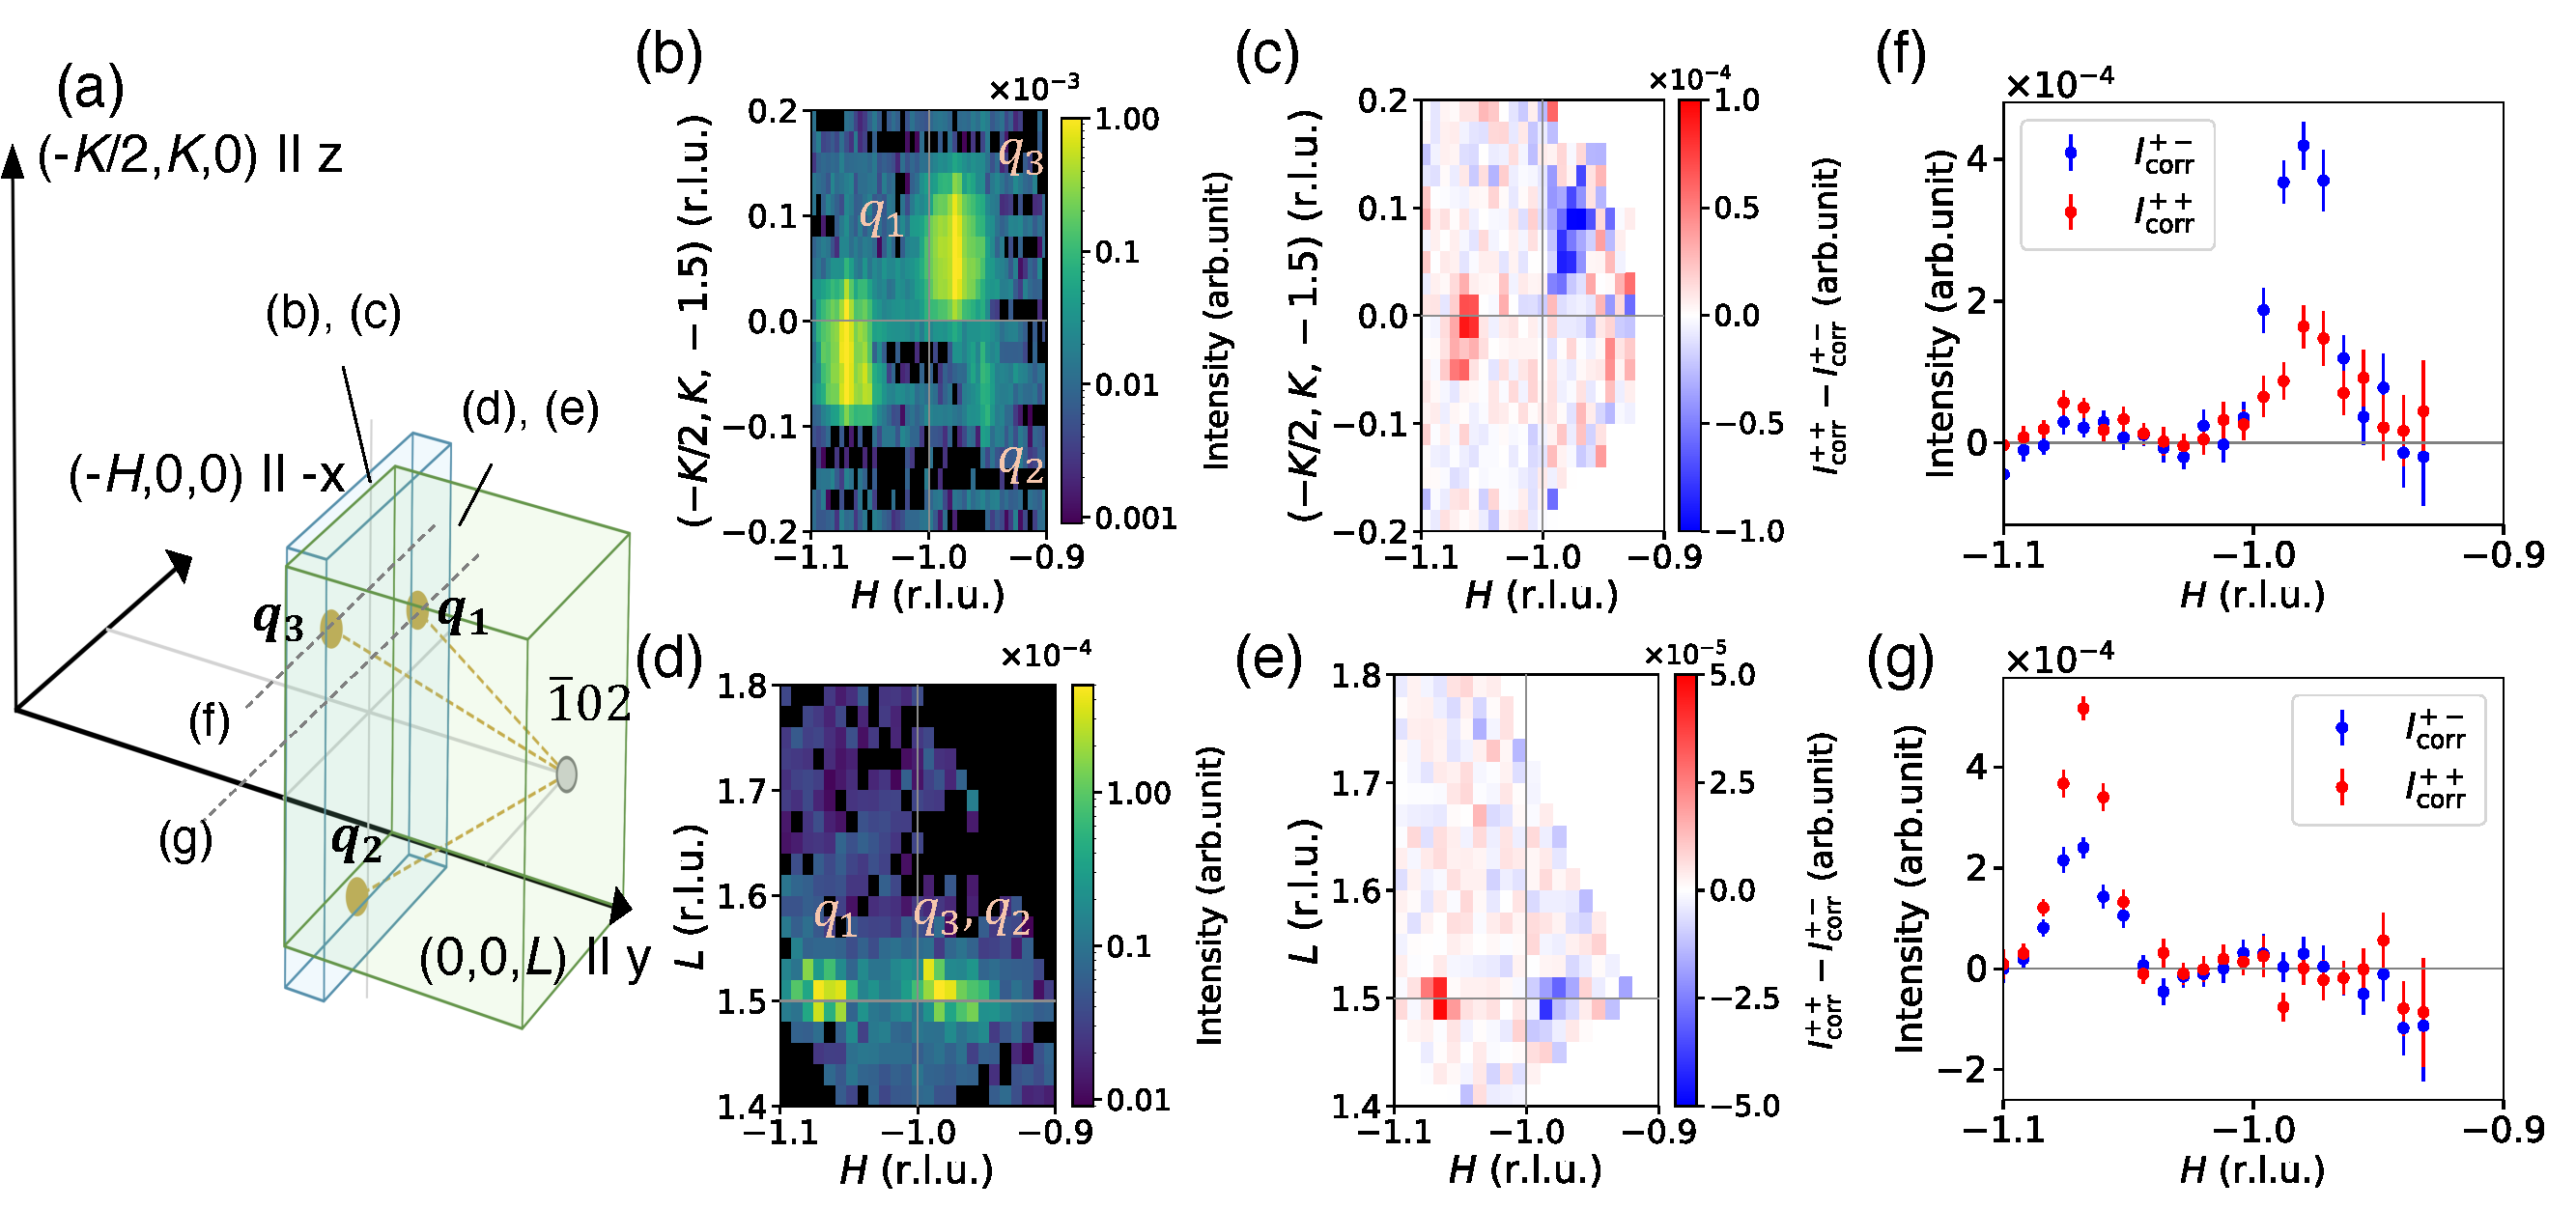
\includegraphics[width=\textwidth]{figure/Figure6_v5.pdf}
    \caption{
\DIFaddFL{(a) Schematic illustration of the reciprocal-space region measured in the present experiment.
The translucent volumes labeled (b), (c) and (d), (e) indicate the regions integrated along the \(L\) direction and the \((-K/2,K,0)\) direction, respectively.
The dashed lines along the \(-H\) direction through \(\boldsymbol{q}_3\) and \(\boldsymbol{q}_1\) indicate the line cuts shown in panels (f) and (g), respectively.
(b), (d) Unpolarized neutron intensity maps in the \((H,K/2,-1.5)\) and \((H,0,L)\) planes, respectively.
(c), (e) Polarization-analysis maps obtained from the difference between the corrected non-spin-flip and corrected spin-flip intensities, \(I^{++}_\mathrm{corr}-I^{+-}_\mathrm{corr}\).
(f), (g) Line profiles of the ($I^{++}_\mathrm{corr}$) and the ($I^{+-}_\mathrm{corr}$) at \(\boldsymbol{q}_3\) and \(\boldsymbol{q}_1\), respectively.
}}
    \label{fig:measured_Qregion}
\end{figure*}


\DIFaddend The polarization of the Heusler polarizer, $P_p$, was also determined from the \DIFdelbegin \DIFdel{same nuclear reflectiondata}\DIFdelend \DIFaddbegin \DIFadd{integrated intensities of the nuclear reflection}\DIFaddend .
From Eqs.~\ref{eq:int_obs_pp} and \ref{eq:int_obs_pm}, the asymmetry between \DIFdelbegin \DIFdel{$I^{++}_\mathrm{obs}$ and $I^{+-}_\mathrm{obs}$ }\DIFdelend \DIFaddbegin \DIFadd{$\mathcal{I}^{++}_\mathrm{obs}$ and $\mathcal{I}^{+-}_\mathrm{obs}$ }\DIFaddend is given by
\begin{equation}
    \DIFdelbegin \DIFdel{\frac{I^{++}_\mathrm{obs}-I^{+-}_\mathrm{obs}}{I^{++}_\mathrm{obs}+I^{+-}_\mathrm{obs}} }\DIFdelend \DIFaddbegin \DIFadd{\frac{\mathcal{I}^{++}_\mathrm{obs}-\mathcal{I}^{+-}_\mathrm{obs}}{\mathcal{I}^{++}_\mathrm{obs}+\mathcal{I}^{+-}_\mathrm{obs}} }\DIFaddend = P_pP_a(t).
\end{equation}
Since $P_a(t)$ \DIFdelbegin \DIFdel{is independently }\DIFdelend \DIFaddbegin \DIFadd{has been already }\DIFaddend determined from the \He polarization, $P_p$ can be obtained from this \DIFdelbegin \DIFdel{relation.
The average }\DIFdelend \DIFaddbegin \DIFadd{equation.
We averaged the }\DIFaddend value of $P_p$ \DIFdelbegin \DIFdel{was found }\DIFdelend \DIFaddbegin \DIFadd{deduced from the measurements of the nuclear reflection, and  $P_p$ was determined }\DIFaddend to be $0.86 \pm 0.06$.
Note that $P_p$ includes the effects of environmental background and neutron depolarization in the guide field.

\DIFdelbegin \DIFdel{The }\DIFdelend \DIFaddbegin \DIFadd{To check the }\DIFaddend validity of the polarization correction \DIFdelbegin \DIFdel{(Eq. ~\ref{eq:int_corr}) was confirmed using the $\omega$ scan of }\DIFdelend \DIFaddbegin \DIFadd{in Eq. 3 and \ref{eq:int_corr}, we measured the intensity distributions near }\DIFaddend the $\bar{1}02$ reflection \DIFaddbegin \DIFadd{with varying the $\omega$ angle}\DIFaddend .
% Fig.6 (a)の説明→(b)の説明。
\DIFdelbegin \DIFdel{At each $\omega$, the intensity was integrated within the peak region identified on the 2D detector (}\DIFdelend \DIFaddbegin \DIFadd{In }\DIFaddend Fig.~\ref{fig:rawdata}\DIFdelbegin \DIFdel{).
The raw intensity profiles of the $\bar{1}02$ reflection show a }\DIFdelend \DIFaddbegin \DIFadd{(a), we show the box-integrated intensities when the \He polarization was parallel and antiparallel to the neutron polarization, as functions of $\omega$, without the polarization correction.
A }\DIFaddend finite spin-flip intensity \DIFaddbegin \DIFadd{was observed }\DIFaddend owing to the imperfect neutron polarization\DIFdelbegin \DIFdel{, as shown in Fig. ~\ref{fig:polcorrection}(a).
By applying }\DIFdelend \DIFaddbegin \DIFadd{. %DIF >
Then, we applied }\DIFaddend the polarization correction \DIFdelbegin \DIFdel{using $P_a(t)$, $T_a(t)$, and $P_p$, the }\DIFdelend \DIFaddbegin \DIFadd{to all the observed intensity maps, and converted them to the intensity distribution in the reciprocal space.
Figure \ref{fig:rawdata}(b) shows the profiles of the }\DIFaddend corrected non-spin-flip and spin-flip intensities, \DIFdelbegin \DIFdel{$I^{++}_\mathrm{corr}$ and $I^{+-}_\mathrm{corr}$, were obtained, as shown in Fig.
~\ref{fig:polcorrection}(b).
}\DIFdelend \DIFaddbegin \DIFadd{$I^{++}$ and $I^{+-}$, along the $(H,0,2)$ line, which were sliced from the three dimensional data.
}\DIFaddend Since only the non-spin-flip scattering \DIFdelbegin \DIFdel{cross section $\Sigma^{++}$ }\DIFdelend is expected for nuclear scattering, \DIFdelbegin \DIFdel{the }\DIFdelend \DIFaddbegin \DIFadd{this }\DIFaddend result indicates that the polarization correction was successfully performed.
Details of the polarization correction are described in Appendix~\ref{appendix}.
\DIFdelbegin \DIFdel{These values were used for the polarization correction of the magnetic scattering data.
}\DIFdelend

% This measurement was repeated while changing the sample rotation angle $\omega$ in steps of $0.1^\circ$.

\subsection{Polarization analysis of magnetic scattering}
\DIFdelbegin %DIFDELCMD < \begin{figure*}[t]
%DIFDELCMD <     \centering
%DIFDELCMD <     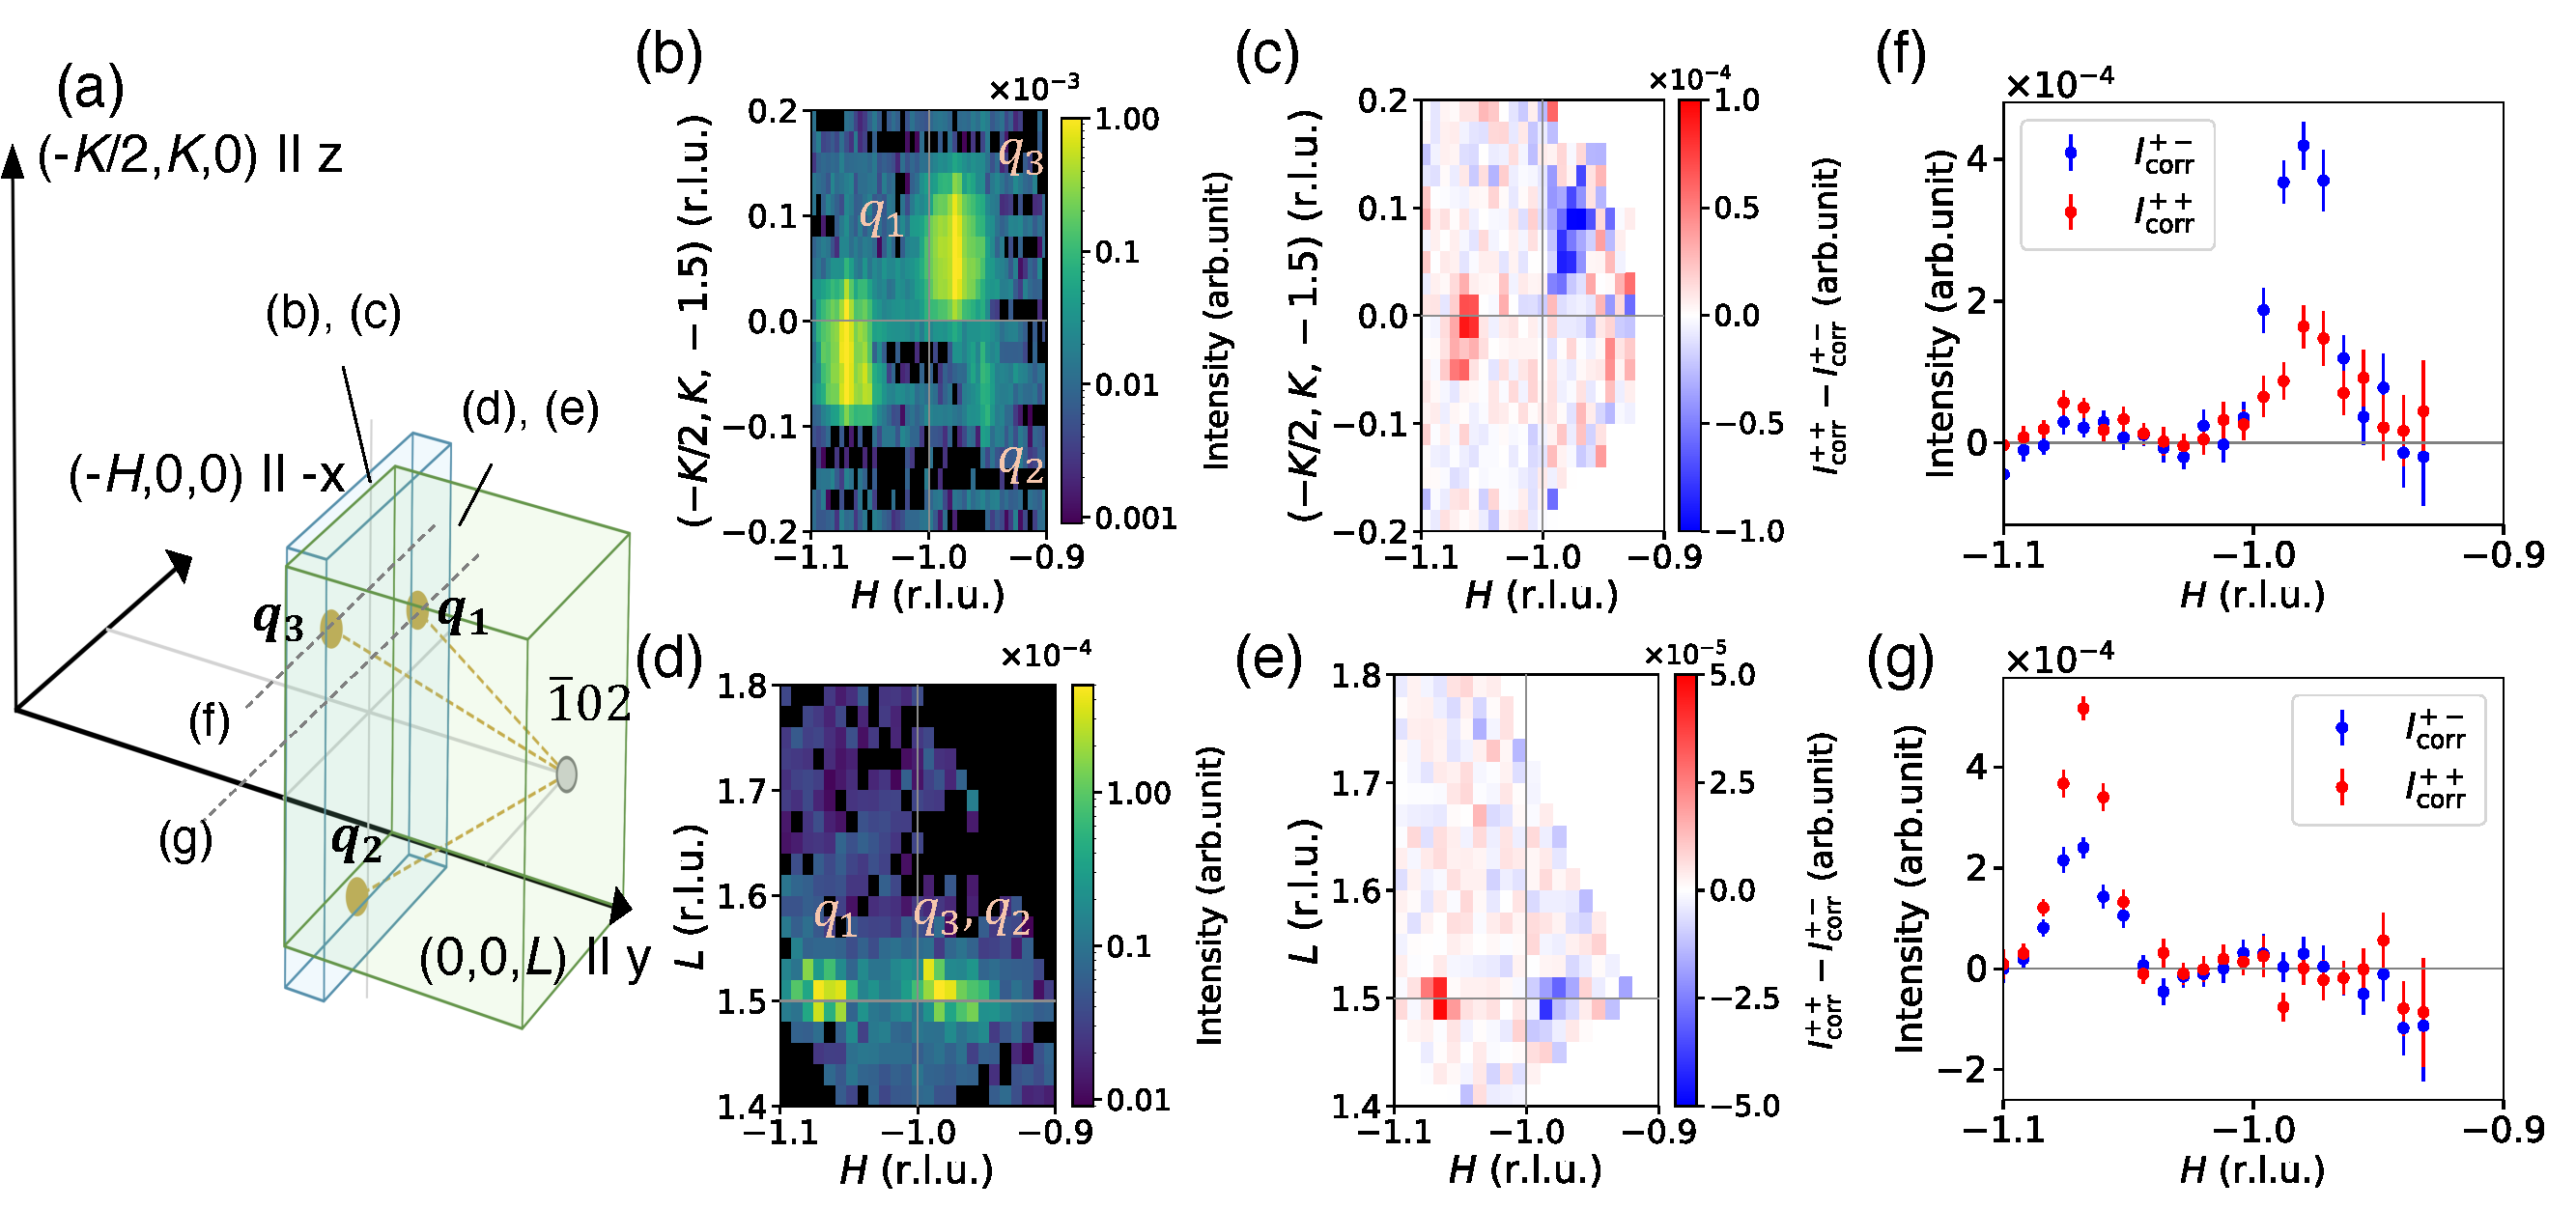
\includegraphics[width=\textwidth]{figure/Figure6_v5.pdf}
%DIFDELCMD <     %%%
%DIFDELCMD < \caption{%
{%DIFAUXCMD
\DIFdelFL{(a) Schematic illustration of the reciprocal-space region measured in the present experiment.
The translucent volumes labeled (b), (c) and (d), (e) indicate the regions integrated along the \(L\) direction and the \((-K/2,K,0)\) direction, respectively.
The dashed lines along the \(-H\) direction through \(\boldsymbol{q}_3\) and \(\boldsymbol{q}_1\) indicate the line cuts shown in panels (f) and (g), respectively.
(b), (d) Unpolarized neutron intensity maps in the \((H,K/2,-1.5)\) and \((H,0,L)\) planes, respectively.
(c), (e) Polarization-analysis maps obtained from the difference between the corrected non-spin-flip and corrected spin-flip intensities, \(I^{++}_\mathrm{corr}-I^{+-}_\mathrm{corr}\).
(f), (g) Line profiles of the ($I^{++}_\mathrm{corr}$) and the ($I^{+-}_\mathrm{corr}$) at \(\boldsymbol{q}_3\) and \(\boldsymbol{q}_1\), respectively.
}}
    %DIFAUXCMD
%DIFDELCMD < \label{fig:measured_Qregion}
%DIFDELCMD < \end{figure*}
%DIFDELCMD < %%%
\DIFdelend

\DIFdelbegin \DIFdel{This subsection presents the polarization-analysis results for the magnetic reflections of  \ce{Mn3WO6}at antiferromagnetic phase .
First, intensity maps of antiferromagnetic reflections were measured using unpolarized neutrons and a }\DIFdelend \DIFaddbegin \DIFadd{We applied the polarized analysis with the \Hensf\ and the }\DIFaddend 2D \DIFaddbegin \DIFadd{detector to the study of magnetic structures of  \ce{Mn3WO6}.
As mentioned in the introduction, this compound exhibits two antiferromagnetically ordered phases. %DIF >
In this paper, we focus on the high temperature phase, and show the data measured at 23 K.
More detailed study including the low temperature phase will be published elsewhere }[\DIFadd{Ref. Osawa}]\DIFadd{.
First, we determined the $q$-vector of the magnetic order by unpolarized neutron diffraction measurements with the 2D }\DIFaddend detector.
The \DIFaddbegin \DIFadd{horizontal }\DIFaddend scattering plane was set to \DIFdelbegin \DIFdel{the \((H0L)\) plane, a conventional triple-axis setup would mainly provide a reciprocal-space map in this plane, }\DIFdelend \DIFaddbegin \DIFadd{be the $(H,0,L)$ plane. %DIF >
We measured the intensity maps with rotating the $\omega$ angle, and converted the data into the reciprocal space. %DIF >
Figure ~\ref{fig:measured_Qregion}(d) shows the intensity distribution projected onto the  \((H0L)\) plane.
We observed two incommensurate reflections near $(-1,0,1.5)$.
To investigate the position of the reflections in more detail, we show the intensity distribution on the $(H,K,1.5)$ plane, which is perpendicular to the horizontal plane, }\DIFaddend as shown in \DIFdelbegin \DIFdel{Fig. ~\ref{fig:measured_Qregion}(d) .
However, the 2D detector enables data analysis along the out-of-plane direction, as demonstrated }\DIFdelend \DIFaddbegin \DIFadd{Figs. \ref{fig:measured_Qregion}(a) and \ref{fig:measured_Qregion}(b), revealing that there are three incommensurate peaks surrounding the $(-1,0,1.5)$.
One of the reflection (labeled $q_1$ }\DIFaddend in Fig. \DIFdelbegin \DIFdel{~}\DIFdelend \ref{fig:measured_Qregion}(b)\DIFdelbegin \DIFdel{.
Here, we can observe the three magnetic reflections }\DIFdelend \DIFaddbegin \DIFadd{) can be indexed by using the $q$-vector of }\DIFaddend $\boldsymbol{q}_1 = (0.059, 0.019, 0.5)$\DIFdelbegin \DIFdel{, and }\DIFdelend \DIFaddbegin \DIFadd{.
Considering the fact that the crystal structure has the threefold rotational symmetry about the $c$ axis, the other two reflections can also be indexed using }\DIFaddend $\boldsymbol{q}_2$ and $\boldsymbol{q}_3$ \DIFdelbegin \DIFdel{correspond to }\DIFdelend \DIFaddbegin \DIFadd{obtained by the }\DIFaddend threefold rotations of $\boldsymbol{q}_1$ about the $c^*$ axis.
\DIFdelbegin \DIFdel{These $\boldsymbol{q}$ values show that }\DIFdelend \DIFaddbegin \DIFadd{Note that the non-equal distribution of the magnetic intensities would be due to the orientations of the Fourier-transformed magnetic moments with respect to the direction of the scattering vector.
We emphasize here that }\DIFaddend $\boldsymbol{q}_1$, $\boldsymbol{q}_2$, and $\boldsymbol{q}_3$ cannot lie within a single 2D plane passing through the reciprocal-space origin \DIFdelbegin \DIFdel{(}\DIFdelend \DIFaddbegin \DIFadd{as shown in }\DIFaddend Fig.~\ref{fig:measured_Qregion}(a)\DIFdelbegin \DIFdel{)}\DIFdelend .
This highlights \DIFdelbegin \DIFdel{why }\DIFdelend \DIFaddbegin \DIFadd{the importance of }\DIFaddend three-dimensional reciprocal-space measurements \DIFdelbegin \DIFdel{are essential for capturing such }\DIFdelend \DIFaddbegin \DIFadd{for elucidating this kind of complex incommensurate }\DIFaddend magnetic structures. %DIF >
\DIFaddbegin

\DIFadd{We thus measured the spin-flip and non-spin-flip intensity distributions around $(-1,0,1.5)$ using the \Hensf.  }\DIFaddend Figures~\ref{fig:measured_Qregion}(c) and \ref{fig:measured_Qregion}(e) show the \DIFdelbegin \DIFdel{polarization-analysis maps obtained from }\DIFdelend the intensity difference \DIFdelbegin \DIFdel{\(I^{++}_\mathrm{corr}-I^{+-}_\mathrm{corr}\).
Clear }\DIFdelend \DIFaddbegin \DIFadd{\(I^{++}-I^{+-}\) mapped onto the $(H,K,1.5)$ and $(H,0,L)$ planes, respectively.
We clearly observed that the difference in intensity takes }\DIFaddend positive and negative \DIFdelbegin \DIFdel{contrasts are observed at the magnetic reflection positions identified in the unpolarized intensity maps.
In addition, to }\DIFdelend \DIFaddbegin \DIFadd{values for the reflection of $\boldsymbol{q}_1$ and $\boldsymbol{q}_3$, respectively.
To }\DIFaddend compare the spin-dependent intensities more quantitatively, line profiles along the \(H\) direction through \(\boldsymbol{q}_3\) and \(\boldsymbol{q}_1\) are shown in Figs.~\ref{fig:measured_Qregion}(f) and \ref{fig:measured_Qregion}(g), respectively.
\DIFdelbegin \DIFdel{The relative intensities of the non-spin-flip }\DIFdelend \DIFaddbegin \DIFadd{At the reflection corresponding to $\boldsymbol{q}_3$, we found that the magnetic scattering intensity was dominated by the spin-flip scattering.
Since the neutron polarization is parallel to the $z$ axis shown in Fig. \ref{fig:measured_Qregion}(a), the spin-flip scattering is attributed to the Fourier-transformed magnetization component on the $xy$ plane, which includes the $a^*$ }\DIFaddend and \DIFaddbegin \DIFadd{$c^*$ axes. %DIF >
At the reflection corresponding to $\boldsymbol{q}_1$, we should observe the Fourier components rotated by 120$^{\circ}$ about the $c$ axis.
If the magnetic structure has only the $c$ component of the magnetic moments, the reflection corresponding to $\boldsymbol{q}_1$ is also dominated by the }\DIFaddend spin-flip \DIFdelbegin \DIFdel{components differ clearly between the two reflections. These polarization-analysis data provide constraints on the magnetic moment components associated with each propagation vector.
A detailed magnetic structure analysis based on these constraints will be presented in a separate paper.
These results indicate that the spin-dependent scatteringintensities were successfully resolved for magnetic reflections distributed in three-dimensional reciprocal space}\DIFdelend \DIFaddbegin \DIFadd{scattering.
However, the observed data show that the non-spin-flip scattering, which is attributed to the $z$ component of the Fourier-transformed magnetization, is stronger for the $\boldsymbol{q}_1$ reflection. %DIF >
This unequivocally demonstrates that the magnetic structure has a finite spin component perpendicular to the $c$ axis. %DIF >
By combining the data measured in other regions of the reciprocal space, the magnetic structure was determined to be an oblique sinusoidal magnetic structure }[\DIFadd{Ref. Osawa}]\DIFaddend . %DIF >
\DIFaddbegin \DIFadd{The present results demonstrated that the polarized neutron scattering with \He cell and 2D detector is quite useful to solve the complex incommensurate magnetic structure.
}\DIFaddend

\section{Summary and Outlook}
In this work, we \DIFdelbegin \DIFdel{developed a polarization analysis method that combines \Hensf~ with a }\DIFdelend \DIFaddbegin \DIFadd{demonstrated polarized neutron diffraction measurements combining \Hensf~ and the }\DIFaddend 2D detector to \DIFdelbegin \DIFdel{analyze arbitrary reciprocal-lattice points distributed in }\DIFdelend \DIFaddbegin \DIFadd{explore }\DIFaddend three-dimensional reciprocal space.
We \DIFdelbegin \DIFdel{demonstrated a }\DIFdelend \DIFaddbegin \DIFadd{established the }\DIFaddend correction procedure for the time-dependent neutron polarization and transmission using a nuclear Bragg reflection and \DIFaddbegin \DIFadd{the NMR signal and }\DIFaddend confirmed its validity.
\DIFdelbegin \DIFdel{Polarization analysis was successfully performed }\DIFdelend \DIFaddbegin \DIFadd{The polarization analysis }\DIFaddend for the incommensurate magnetic reflections of \ce{Mn3WO6} \DIFdelbegin \DIFdel{at antiferromagnetic phase, and the details of the magnetic structure will be reported in a separate paper.
The positions of the \Hensf~and the 2D detector were fixed in the present experiment, whereas a configuration in which both devices are mounted on a scanning arm is planned to cover a wider region of reciprocal space}\DIFdelend \DIFaddbegin \DIFadd{was successfully performed, highlighting the importance of the polarization analysis for the magnetic reflections out of the horizontal plane}\DIFaddend .
Although the present \textit{ex-situ} method requires time-dependent correction, \DIFaddbegin \DIFadd{it is possible to upgrade it to the }\DIFaddend \textit{in-situ} \DIFdelbegin \DIFdel{method unnecessary the time-dependent correction because SEOP is performed continously throughout the measurement on the beampath.
Recently}\DIFdelend \DIFaddbegin \DIFadd{SEOP method.
In fact}\DIFaddend , a compact \textit{in-situ} \Hensf~system has been \DIFaddbegin \DIFadd{recently }\DIFaddend developed at J-PARC\DIFdelbegin \DIFdel{, which can be mounted on a scanning detector arm}\DIFdelend \cite{takahashi_development_2025}.
This implementation is expected to maintain high neutron polarization and transmission throughout the experiment, thereby facilitating polarization analysis of complex magnetic structures over a wider region of reciprocal space and for a broader range of materials.

\begin{acknowledgments}
We thank Mr. Ohkawara (Tohoku Univ.) for his kind support in operating the SEOP laser system in the experimental area.
This work was supported by JSPS KAKENHI Grant Number 25KJ0050.
\end{acknowledgments}

\appendix
\section{Polarization correction with \textit{ex-situ} \He neutron spin filter}
\label{appendix}
In this section, the polarization correction in the present experimental setup is described.
This correction is based on the polarization matrix reported by A. Wildes \cite{wildes_polarizer-analyzer_1999,wildes_scientific_2006}.
A spin-dependent measured count for the non-spin flip configuration ($I^{++}_\mathrm{obs}$) is expressed as follows:
\begin{align}
    I^{++}_\mathrm{obs} &= N_0 T_p p_p \Sigma^{++} T_a p_a \notag \\
    &+ N_0 T_p p_p \Sigma^{+-} T_a (1-p_a) \notag\\
    &+N_0 T_p (1-p_p) \Sigma^{-+} T_a p_a \notag \\
    &+ N_0 T_p (1-p_p) \Sigma^{--} T_a (1-p_a),
    \label{eq:Ipp}
\end{align}
Here, $N_0$ is the total number of incident neutrons, assumed to include equal populations of the ($+$) and ($-$) spin states.
$T_p$ and $T_a$ are the total neutron transmissions of the polarizer and analyzer, respectively.
$p_p$ and $p_a$ are the polarization efficiencies of the polarizer and analyzer, respectively.
$\Sigma^{++}$, $\Sigma^{+-}$, $\Sigma^{-+}$, and $\Sigma^{--}$ are the scattering cross sections for the corresponding spin states.
The derivation of this equation is schematically illustrated in Fig.~\ref{fig:appendix}.
The polarization efficiencies $p_p$ and $p_a$ are defined within the ranges $0.5 \leq p_p \leq 1$ and $0.5 \leq p_a \leq 1$.
In the present experimental setup, only the $I^{++}$ and the $I^{+-}$ configurationscan can be measured.
The chiral contribution and the nuclear-magnetic interference term are assumed to be negligible, such that the scattering cross sections satisfy $\Sigma^{++} = \Sigma^{--}$ and $\Sigma^{+-} = \Sigma^{-+}$.
Under these assumptions, Eq.~\ref{eq:Ipp} can be rewritten into the following matrix form that includes the spin flip configuration:
\begin{equation}
    \begin{bmatrix}
        I^{++}_\mathrm{obs} \\
        I^{+-}_\mathrm{obs}
    \end{bmatrix}
    =
    N_0T_pT_a
    \begin{bmatrix}
        p_p & 1-p_p \\
        1-p_p & p_p \\
    \end{bmatrix}
    \begin{bmatrix}
        p_a&1-p_a \\
        1-p_a&p_a \\
    \end{bmatrix}
    \begin{bmatrix}
        \Sigma^{++} \\
        \Sigma^{+-}
    \end{bmatrix}.
    \label{eq:Ipp_Ipm}
\end{equation}

Since the \textit{ex-situ} \Hensf~exhibits a decay of the \He polarization over time, both the neutron polarization efficiency $p_a$ and the neutron transmission $T_a$ become time-dependent.
Accordingly, by treating Eq.~\ref{eq:Ipp_Ipm} as a time-dependent matrix equation and taking its inverse, the following expression is obtained:
\begin{widetext}
    \begin{align}
        \begin{bmatrix}
            \Sigma^{++} \\
            \Sigma^{+-}
        \end{bmatrix}
        &=\frac{1}{N_0T_pP_p\left(P_a(t_1)+P_a(t_2)\right)}
        \begin{bmatrix}
        1+P_pP_a(t_2) & -1+P_pP_a(t_1) \\
        -1+P_pP_a(t_2) & 1+P_pP_a(t_1)
        \end{bmatrix}
        \begin{bmatrix}
        1/T_a(t_1) & 0 \\
        0 & 1/T_a(t_2)
        \end{bmatrix}
        \begin{bmatrix}
            I^{++}_\mathrm{obs}(t_1) \\
            I^{+-}_\mathrm{obs}(t_2)
        \end{bmatrix},
    \label{eq:Sigma}
    \end{align}
\end{widetext}
where $p_p$ and $p_a$ are converted to $P_p$ and $P_a$ using the relations $P_p = 2p_p -1$ and $P_a = 2p_a -1$.
$T_a(t)$, $P_p$, and $P_a(t)$ are experimentally determined and described in Sec.~\ref{sec:He-3}.
In the main text, $N_0$ and $T_p$ are treated as a scale factor and are absorbed into the corrected intensities $I^{+\pm}_\mathrm{corr}$.

\begin{figure}[t]
    \centering
    \DIFdelbeginFL %DIFDELCMD < 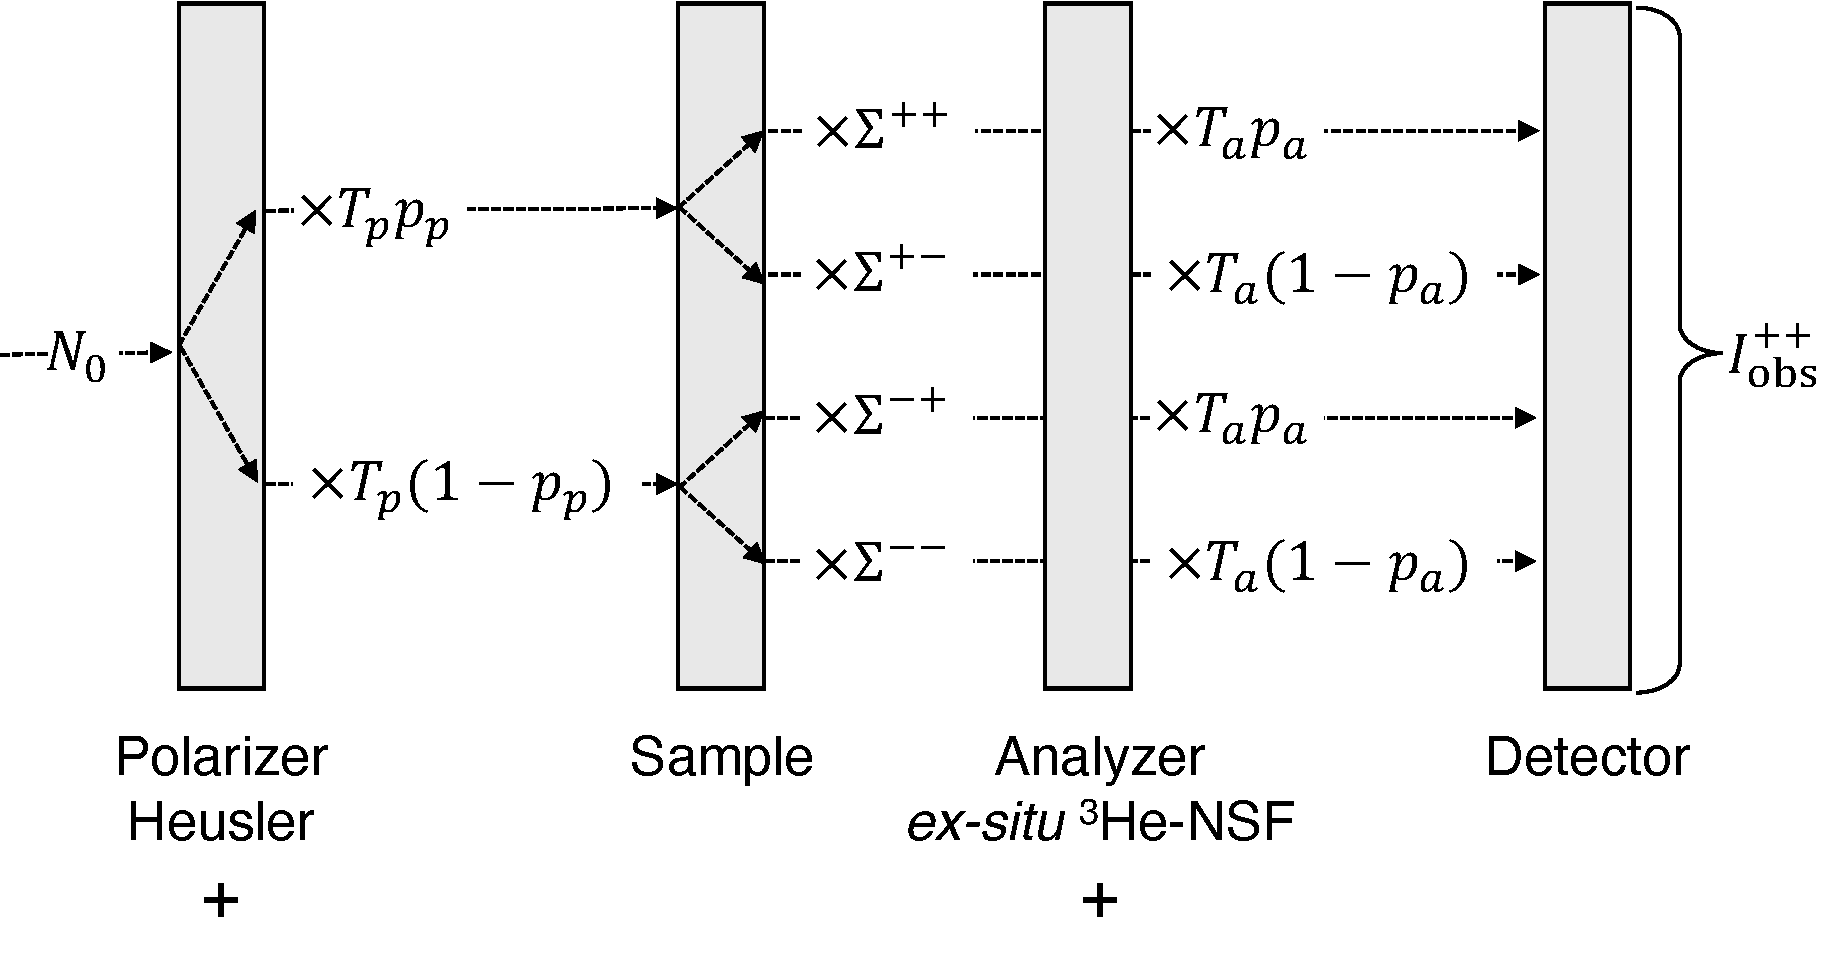
\includegraphics[width=8.5cm]{figure/Appendix_v7.pdf}
%DIFDELCMD <     %%%
\DIFdelendFL \DIFaddbeginFL 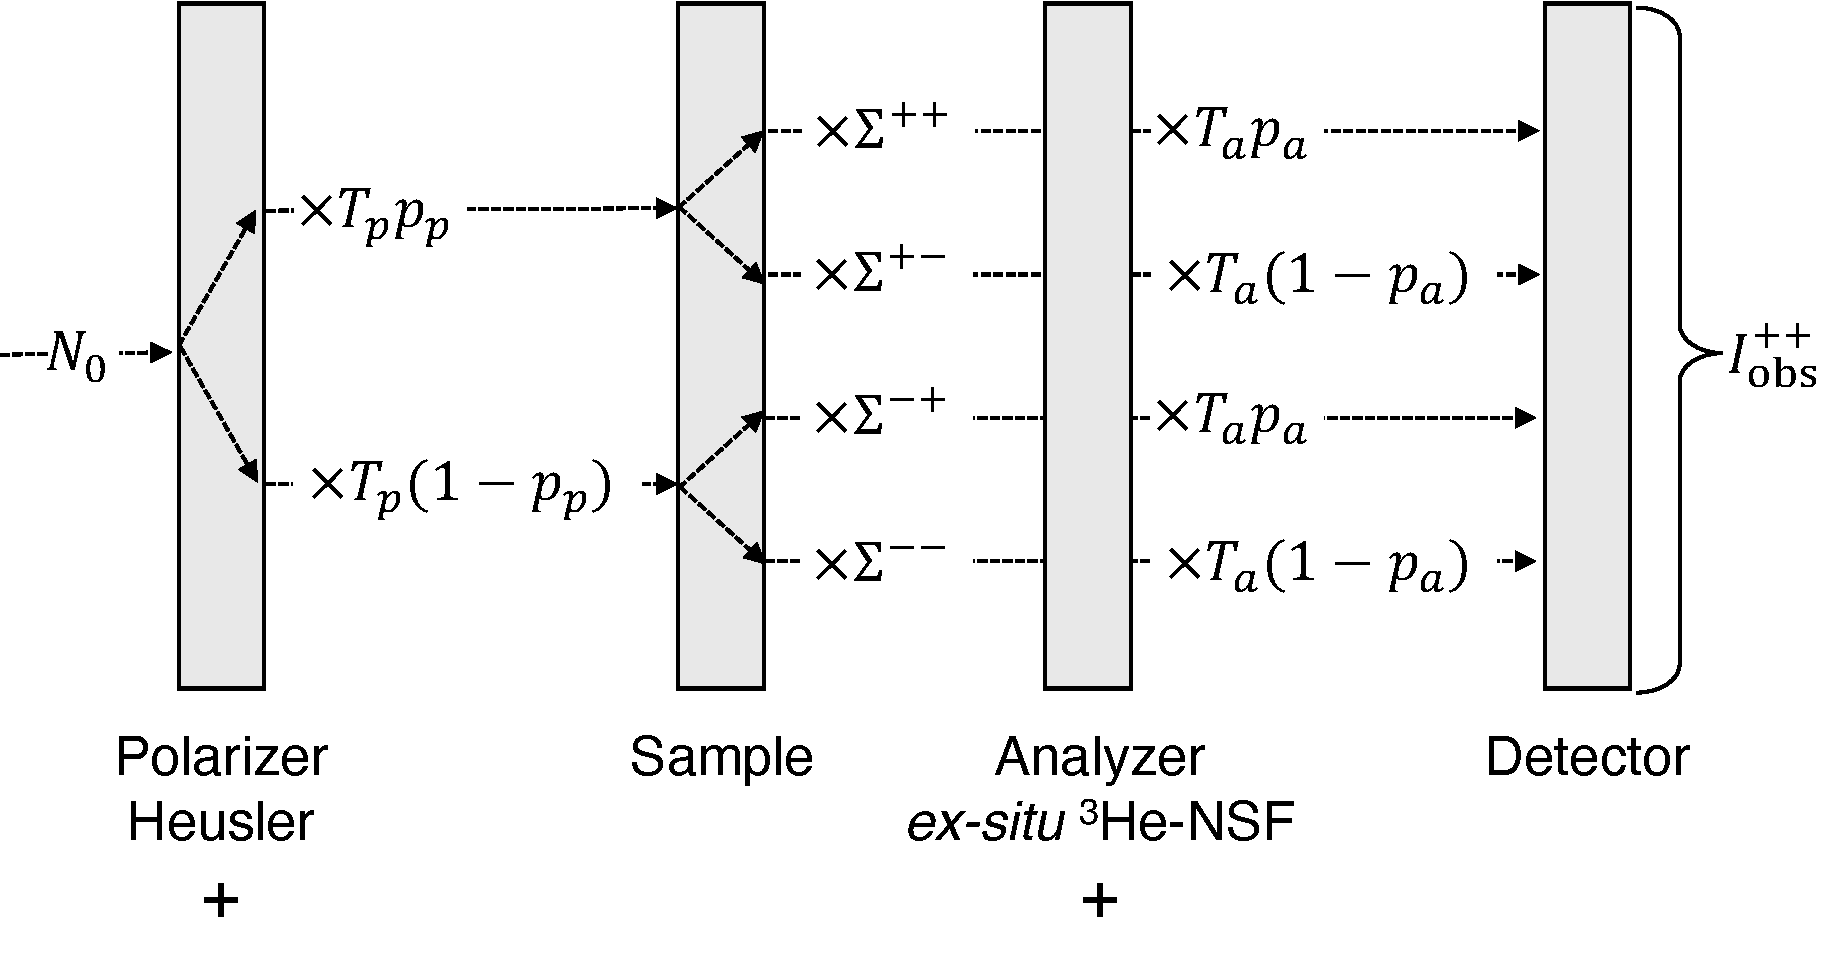
\includegraphics[width=8.5cm]{figure/Appendix_v7.pdf}
    \DIFaddendFL \caption{Schematic diagram of the spin-dependent neutron intensity in the present experimental setup.
    The measured intensity $I^{++}$ is given by the sum of the contributions from the four spin-scattering channels when the Heusler crystal and the \Hensf~are both polarized in the same direction.}
    \label{fig:appendix}
\end{figure}




\bibliographystyle{apsrev4-2}
\bibliography{ref}

\end{document}
%
% ****** End of file apssamp.tex ******
